\subsection{SM and beyond}

\begin{frame}{\Tp~pair production}
\vspace{-.2cm}
\begin{figure}[!Hhtbp]
  \begin{center}
    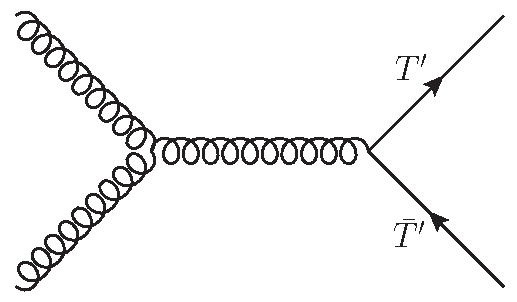
\includegraphics[width=0.3\textwidth]{../figs/Gluon_fusion_T_pair.jpg}
    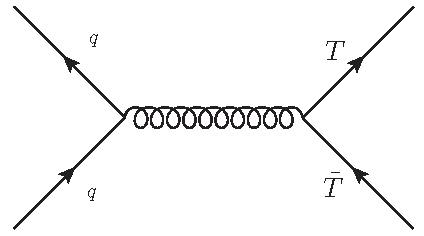
\includegraphics[width=0.3\textwidth]{../figs/Quarks_schannel_T_pair.jpg}
    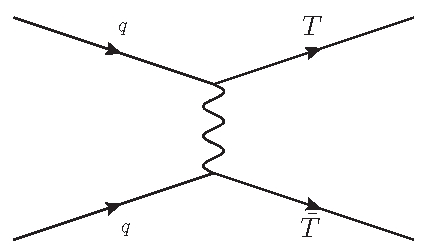
\includegraphics[width=0.3\textwidth]{../figs/Gluon_tchannel_T_pair.jpg}
    %\caption{Feynman diagrams of \Tp~production in pairs.}
    %\label{fig:ProdDiagPair}
  \end{center}
\end{figure}

\vspace{-.2cm}
    \begin{block}{}
      \tiny \centering Feynman diagrams of \Tp~production in pairs.
    \end{block}

\end{frame}

\begin{frame}{\Tp~single production}
\vspace{-.2cm}
\begin{figure}[!Hhtbp]
  \begin{center}
    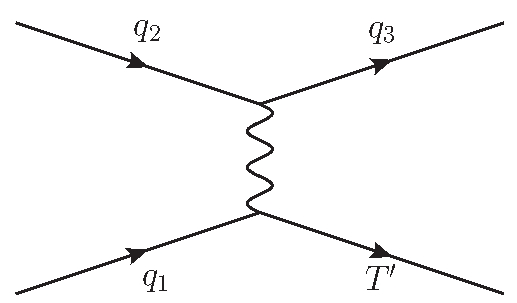
\includegraphics[width=0.45\textwidth]{../figs/Tchannel_T_single.jpg}
    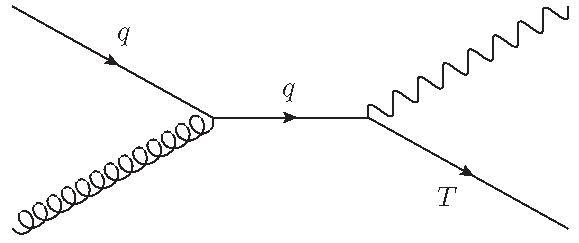
\includegraphics[width=0.45\textwidth]{../figs/QuarkGluonFusion_SingleT.jpg}
    %\caption{Single \Tp~production Feynman diagrams.}
    %\label{fig:ProdDiagSingle}
  \end{center}
\end{figure}

\vspace{-.2cm}
    \begin{block}{}
      \tiny \centering Single \Tp~production Feynman diagrams.
    \end{block}

\end{frame}

\begin{frame}{\Tp~branching ratios}
\vspace{-.2cm}
\begin{figure}[!Hhtbp]
  \begin{center}
    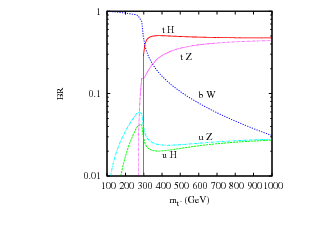
\includegraphics[width=0.6\textwidth]{../figs/pheno_br_tp.png}
    %\caption{\Tp~branching ratios as a function of its mass~\cite{Cacciapaglia:2011fx}.}
    %\label{fig:TBRs}
  \end{center}
\end{figure}

\vspace{-.2cm}
    \begin{block}{}
      \tiny \centering \Tp~branching ratios as a function of its mass.
    \end{block}

\end{frame}

\begin{frame}{Top quark pair production}
\vspace{-.2cm}
\begin{figure}[!Hhtbp]
  \begin{center}
    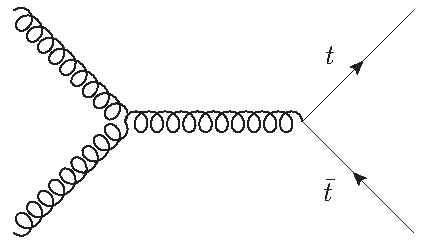
\includegraphics[width=0.32\textwidth]{../figs/Gluon_fusion_top_pair.jpg}
    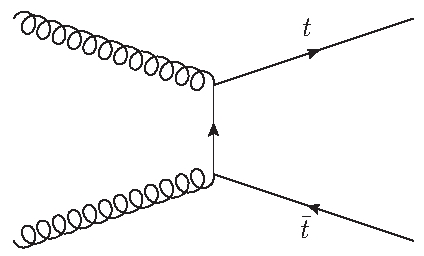
\includegraphics[width=0.32\textwidth]{../figs/Gluon_tchannel_top_pair.jpg}
    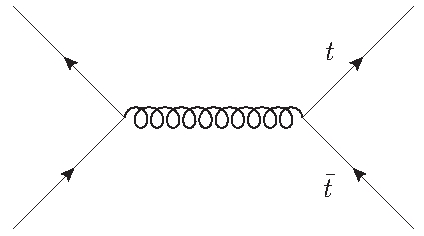
\includegraphics[width=0.32\textwidth]{../figs/Quarks_schannel_top_pair.jpg}
    %\caption{Top pair production processes Feynman diagrams for proton-proton collisions, via gluon fusion [left], gluon t-channel [middle] and quark-antiquark annihilation [right].}
    %\label{fig:PairProductionFD}
  \end{center}
\end{figure}

\vspace{-.2cm}
    \begin{block}{}
      \tiny \centering Top pair production processes Feynman diagrams for proton-proton collisions, via gluon fusion [left], gluon t-channel [middle] and quark-antiquark annihilation [right].
    \end{block}

\end{frame}

\begin{frame}{Top quark single production}
\vspace{-.2cm}
\begin{figure}[!Hhtbp]
  \begin{center}
    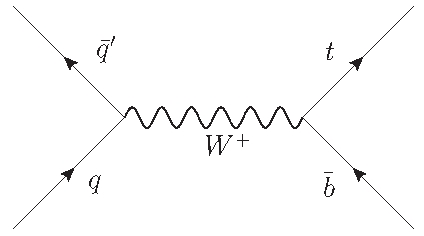
\includegraphics[width=0.32\textwidth]{../figs/Schannel_top_single.jpg}
    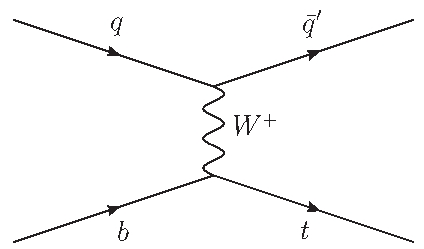
\includegraphics[width=0.32\textwidth]{../figs/Tchannel_top_single.jpg}
    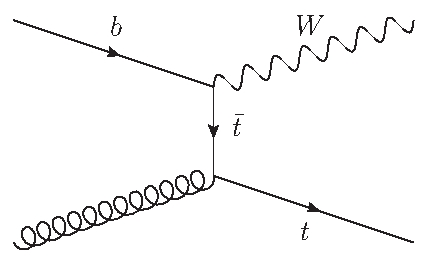
\includegraphics[width=0.32\textwidth]{../figs/TWchannel_top_single.jpg}
    %\caption{Feynman diagrams of single top production processes of proton-proton collisions, from left to right s-channel, t-channel and associated \W~production.}
    %\label{fig:SingleProductionFD}
  \end{center}
\end{figure}

\vspace{-.2cm}
    \begin{block}{}
      \tiny \centering Feynman diagrams of single top production processes of proton-proton collisions, from left to right s-channel, t-channel and associated \W~production.
    \end{block}

\end{frame}

\begin{frame}{}
\vspace{-.2cm}
\begin{figure}[!Hhtbp]
  \begin{center}
    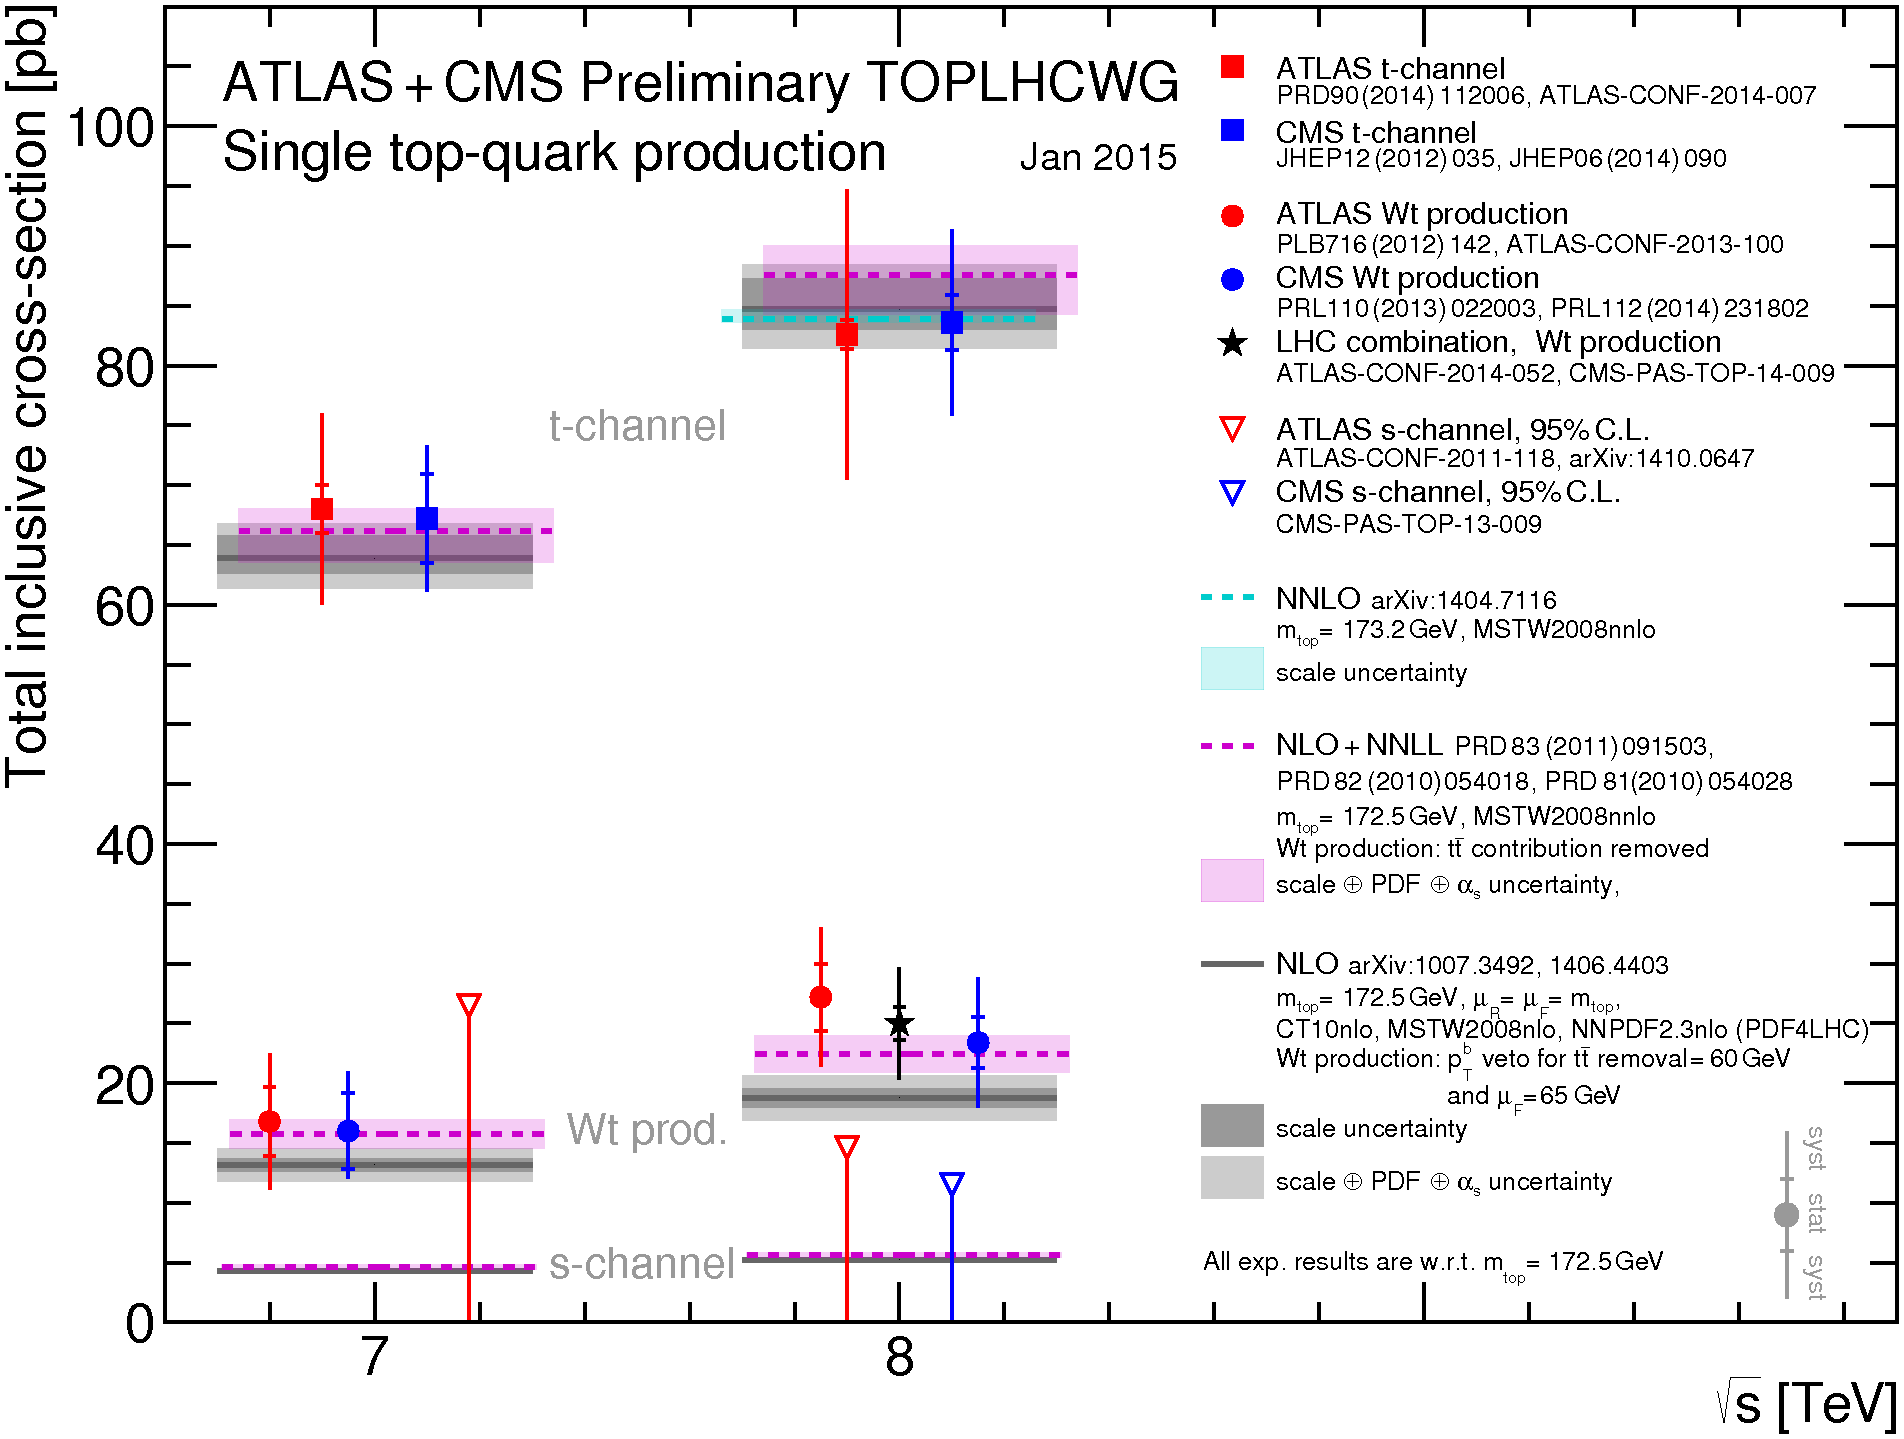
\includegraphics[width=0.9\textwidth]{../figs/singletop_allchanvsroots.png}
    %\caption{Single top production cross section as a function of the center of mass energy in proton-proton collisions compared to theoretical predictions for each production channel by ATLAS and CMS collaborations~\cite{TOPLHCWG}.}
    %\label{fig:SingleProduction}
  \end{center}
\end{figure}

\vspace{-.2cm}
    \begin{block}{}
      \tiny \centering Single top production cross section as a function of the center of mass energy in proton-proton collisions compared to theoretical predictions for each production channel by ATLAS and CMS collaborations.
    \end{block}

\end{frame}

\begin{frame}{Top Decay}
\vspace{-.2cm}
\begin{figure}[!Hhtbp]
  \begin{center}
    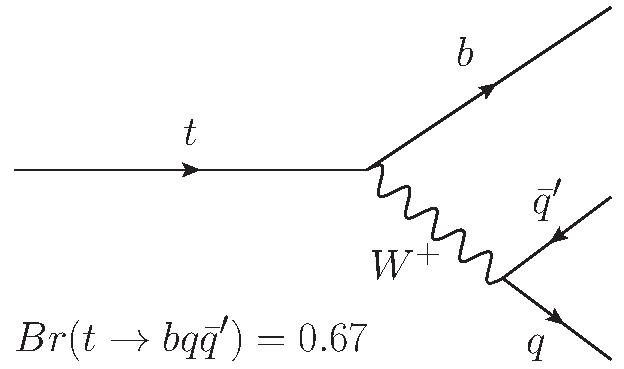
\includegraphics[width=0.4\textwidth]{../figs/Top_H_Decay.png}
    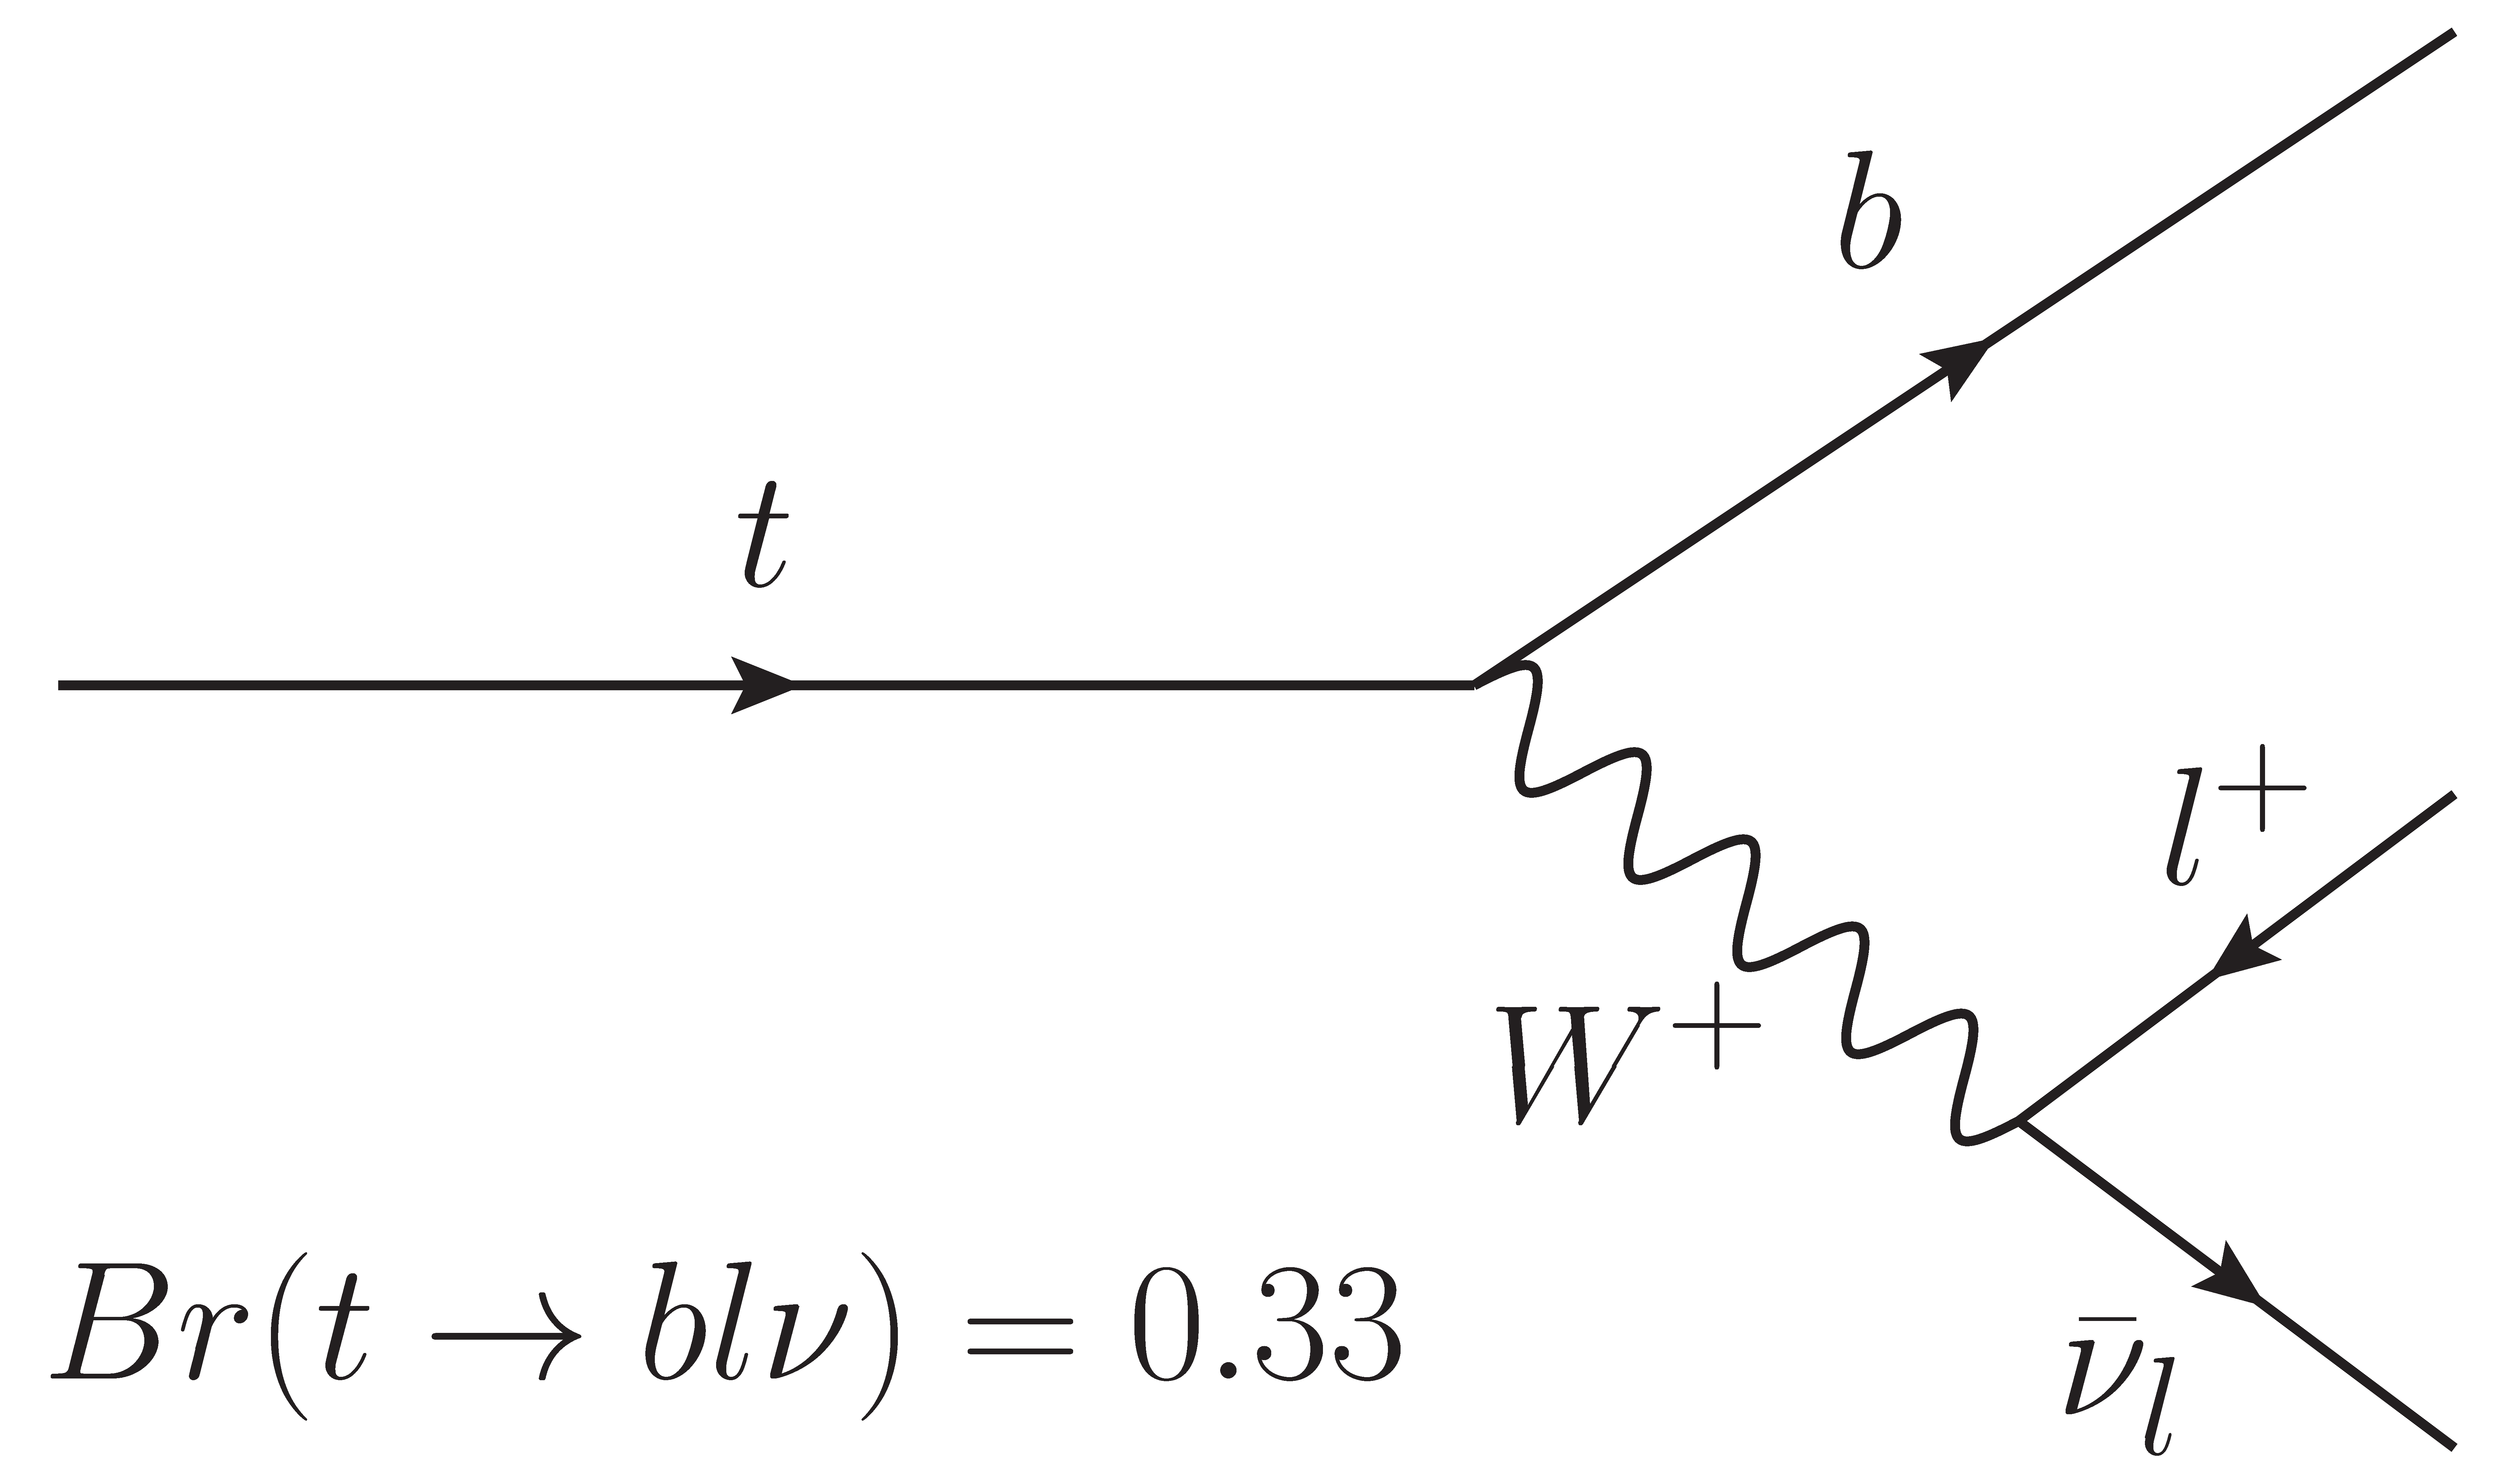
\includegraphics[width=0.4\textwidth]{../figs/Top_L_Decay.png}
    %\caption{Feynman diagrams for top decay channels with respective branching ratios.}
    %\label{fig:BRratiosandDecayChannels}
  \end{center}
\end{figure}

\vspace{-.2cm}
    \begin{block}{}
      \tiny \centering Feynman diagrams for top decay channels with respective branching ratios.
    \end{block}

\end{frame}

\begin{frame}{Top mass}
\vspace{-.2cm}
\begin{figure}[!Hhtbp]
  \begin{center}
    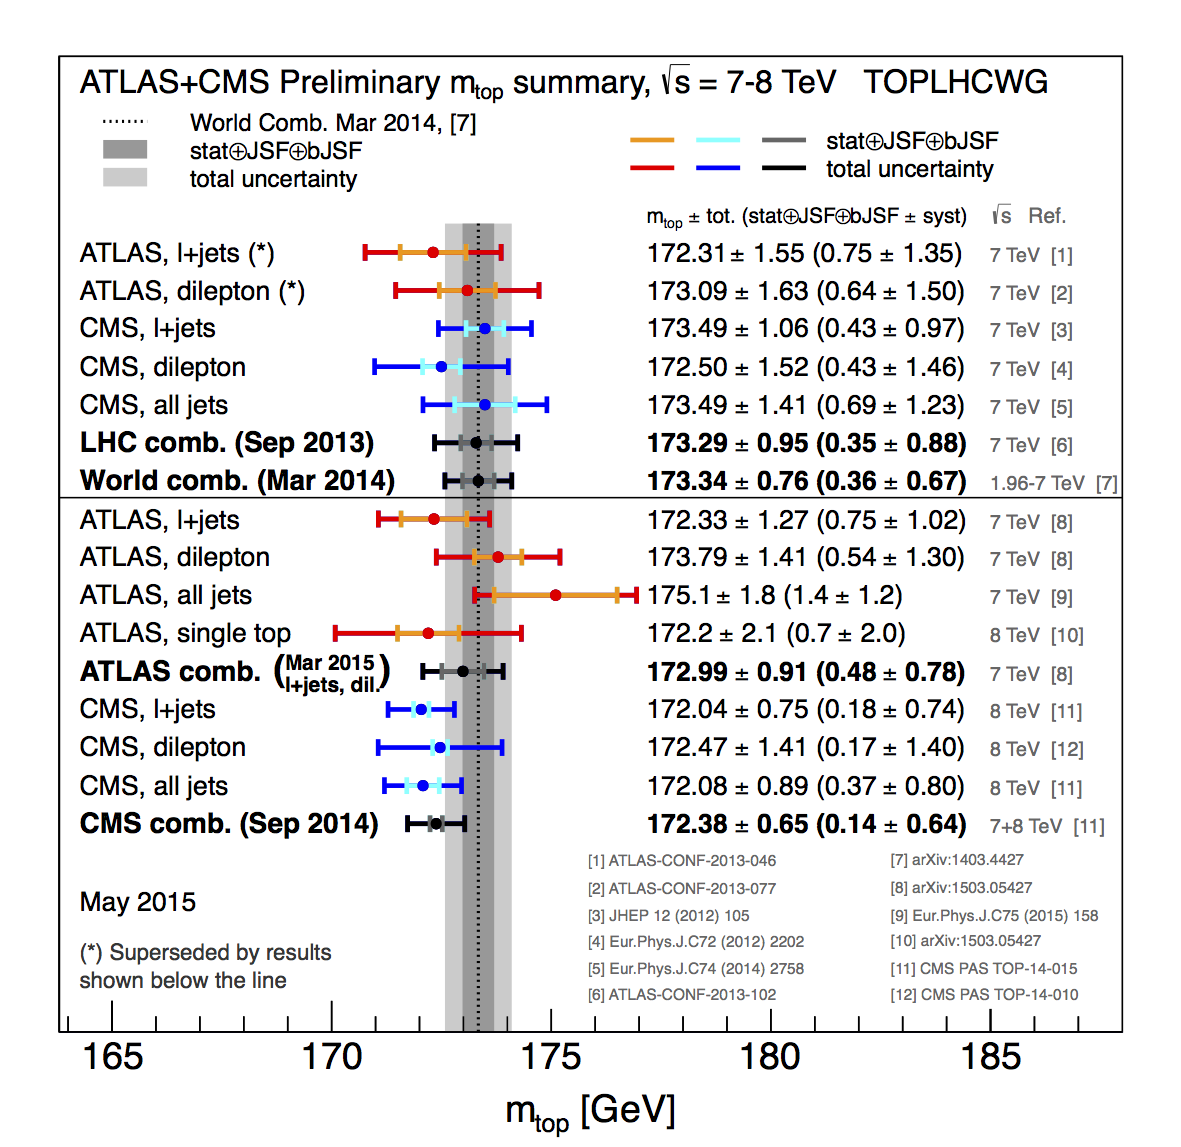
\includegraphics[width=0.6\textwidth]{../figs/LHC_topmass_May2015.png}
    %\caption{Top mass measurements from ATLAS and CMS collaborations and world combination including Tevatron results~\cite{TOPLHCWG}.}
    %\label{fig:TopMass}
  \end{center}
\end{figure}


\vspace{-.2cm}
    \begin{block}{}
      \tiny \centering Top mass measurements from ATLAS and CMS collaborations and world combination including Tevatron results.
    \end{block}

\end{frame}

\begin{frame}{Higgs production}
\vspace{-.2cm}
\begin{figure}[!Hhtbp]
  \begin{center}
    \includegraphics[width=0.35\textwidth, height=3.cm]{../figs/GluonFusion_H.png}
    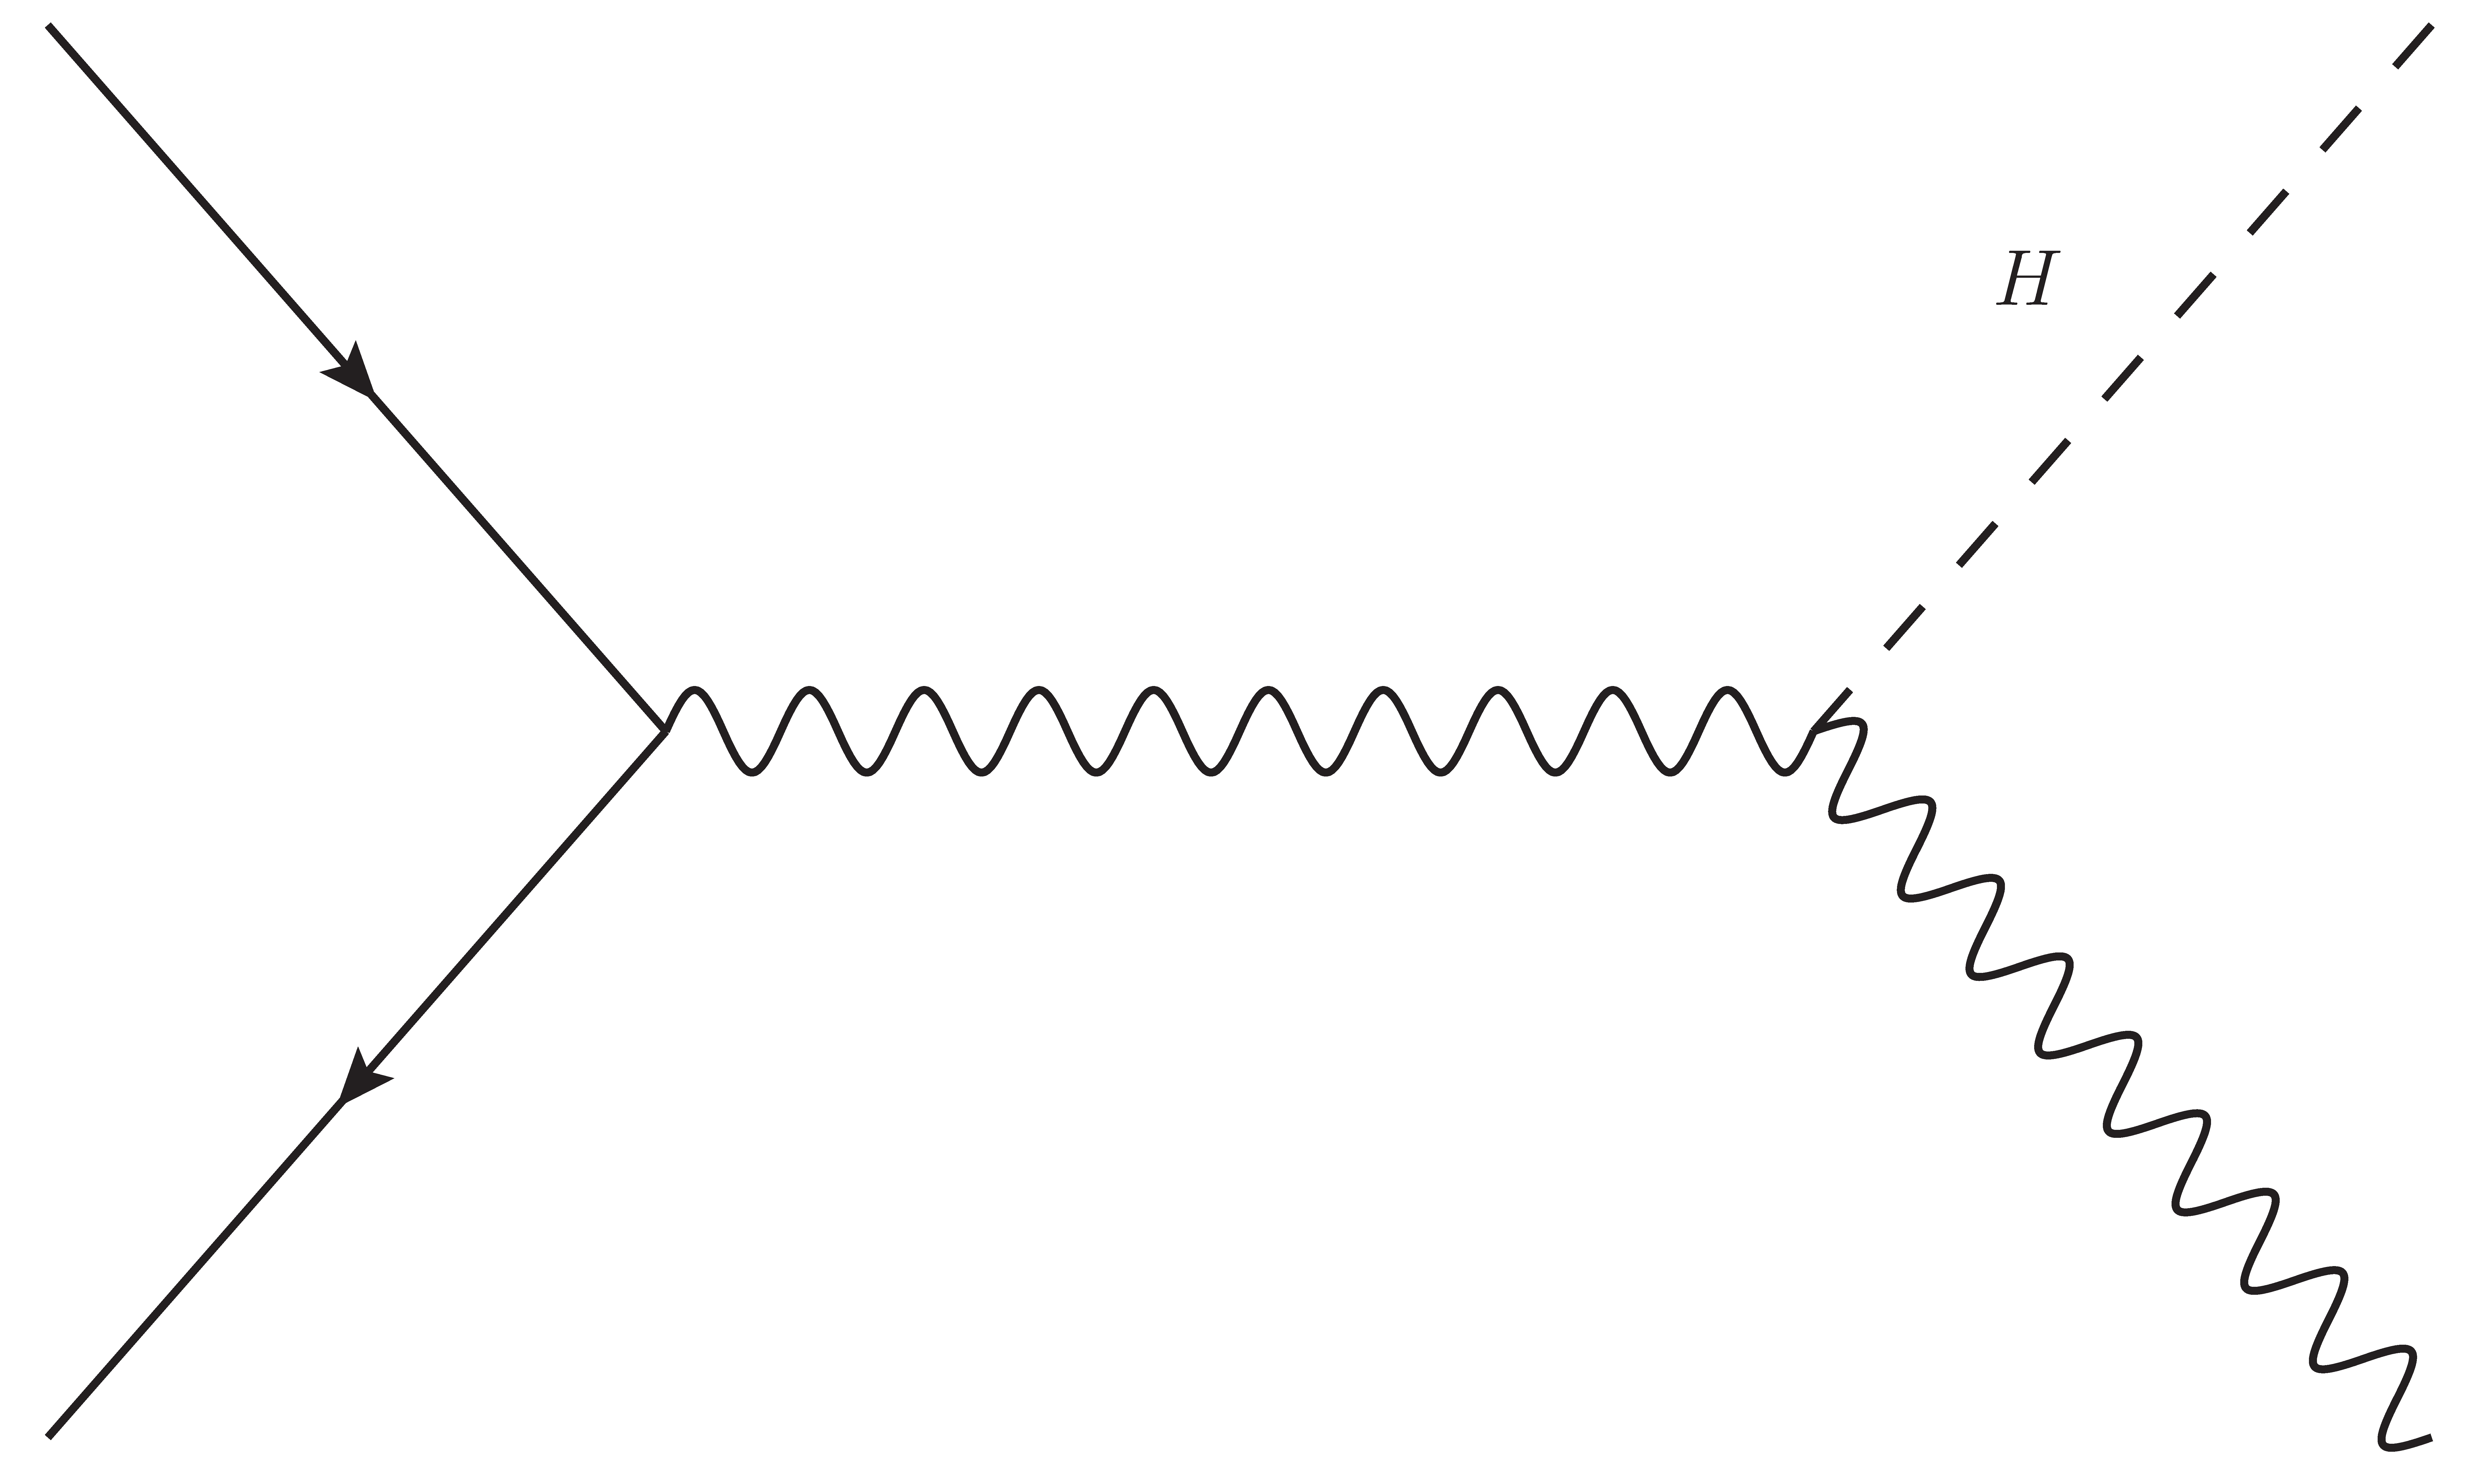
\includegraphics[width=0.35\textwidth, height=3.cm]{../figs/Higgstrahlung.png}\\
    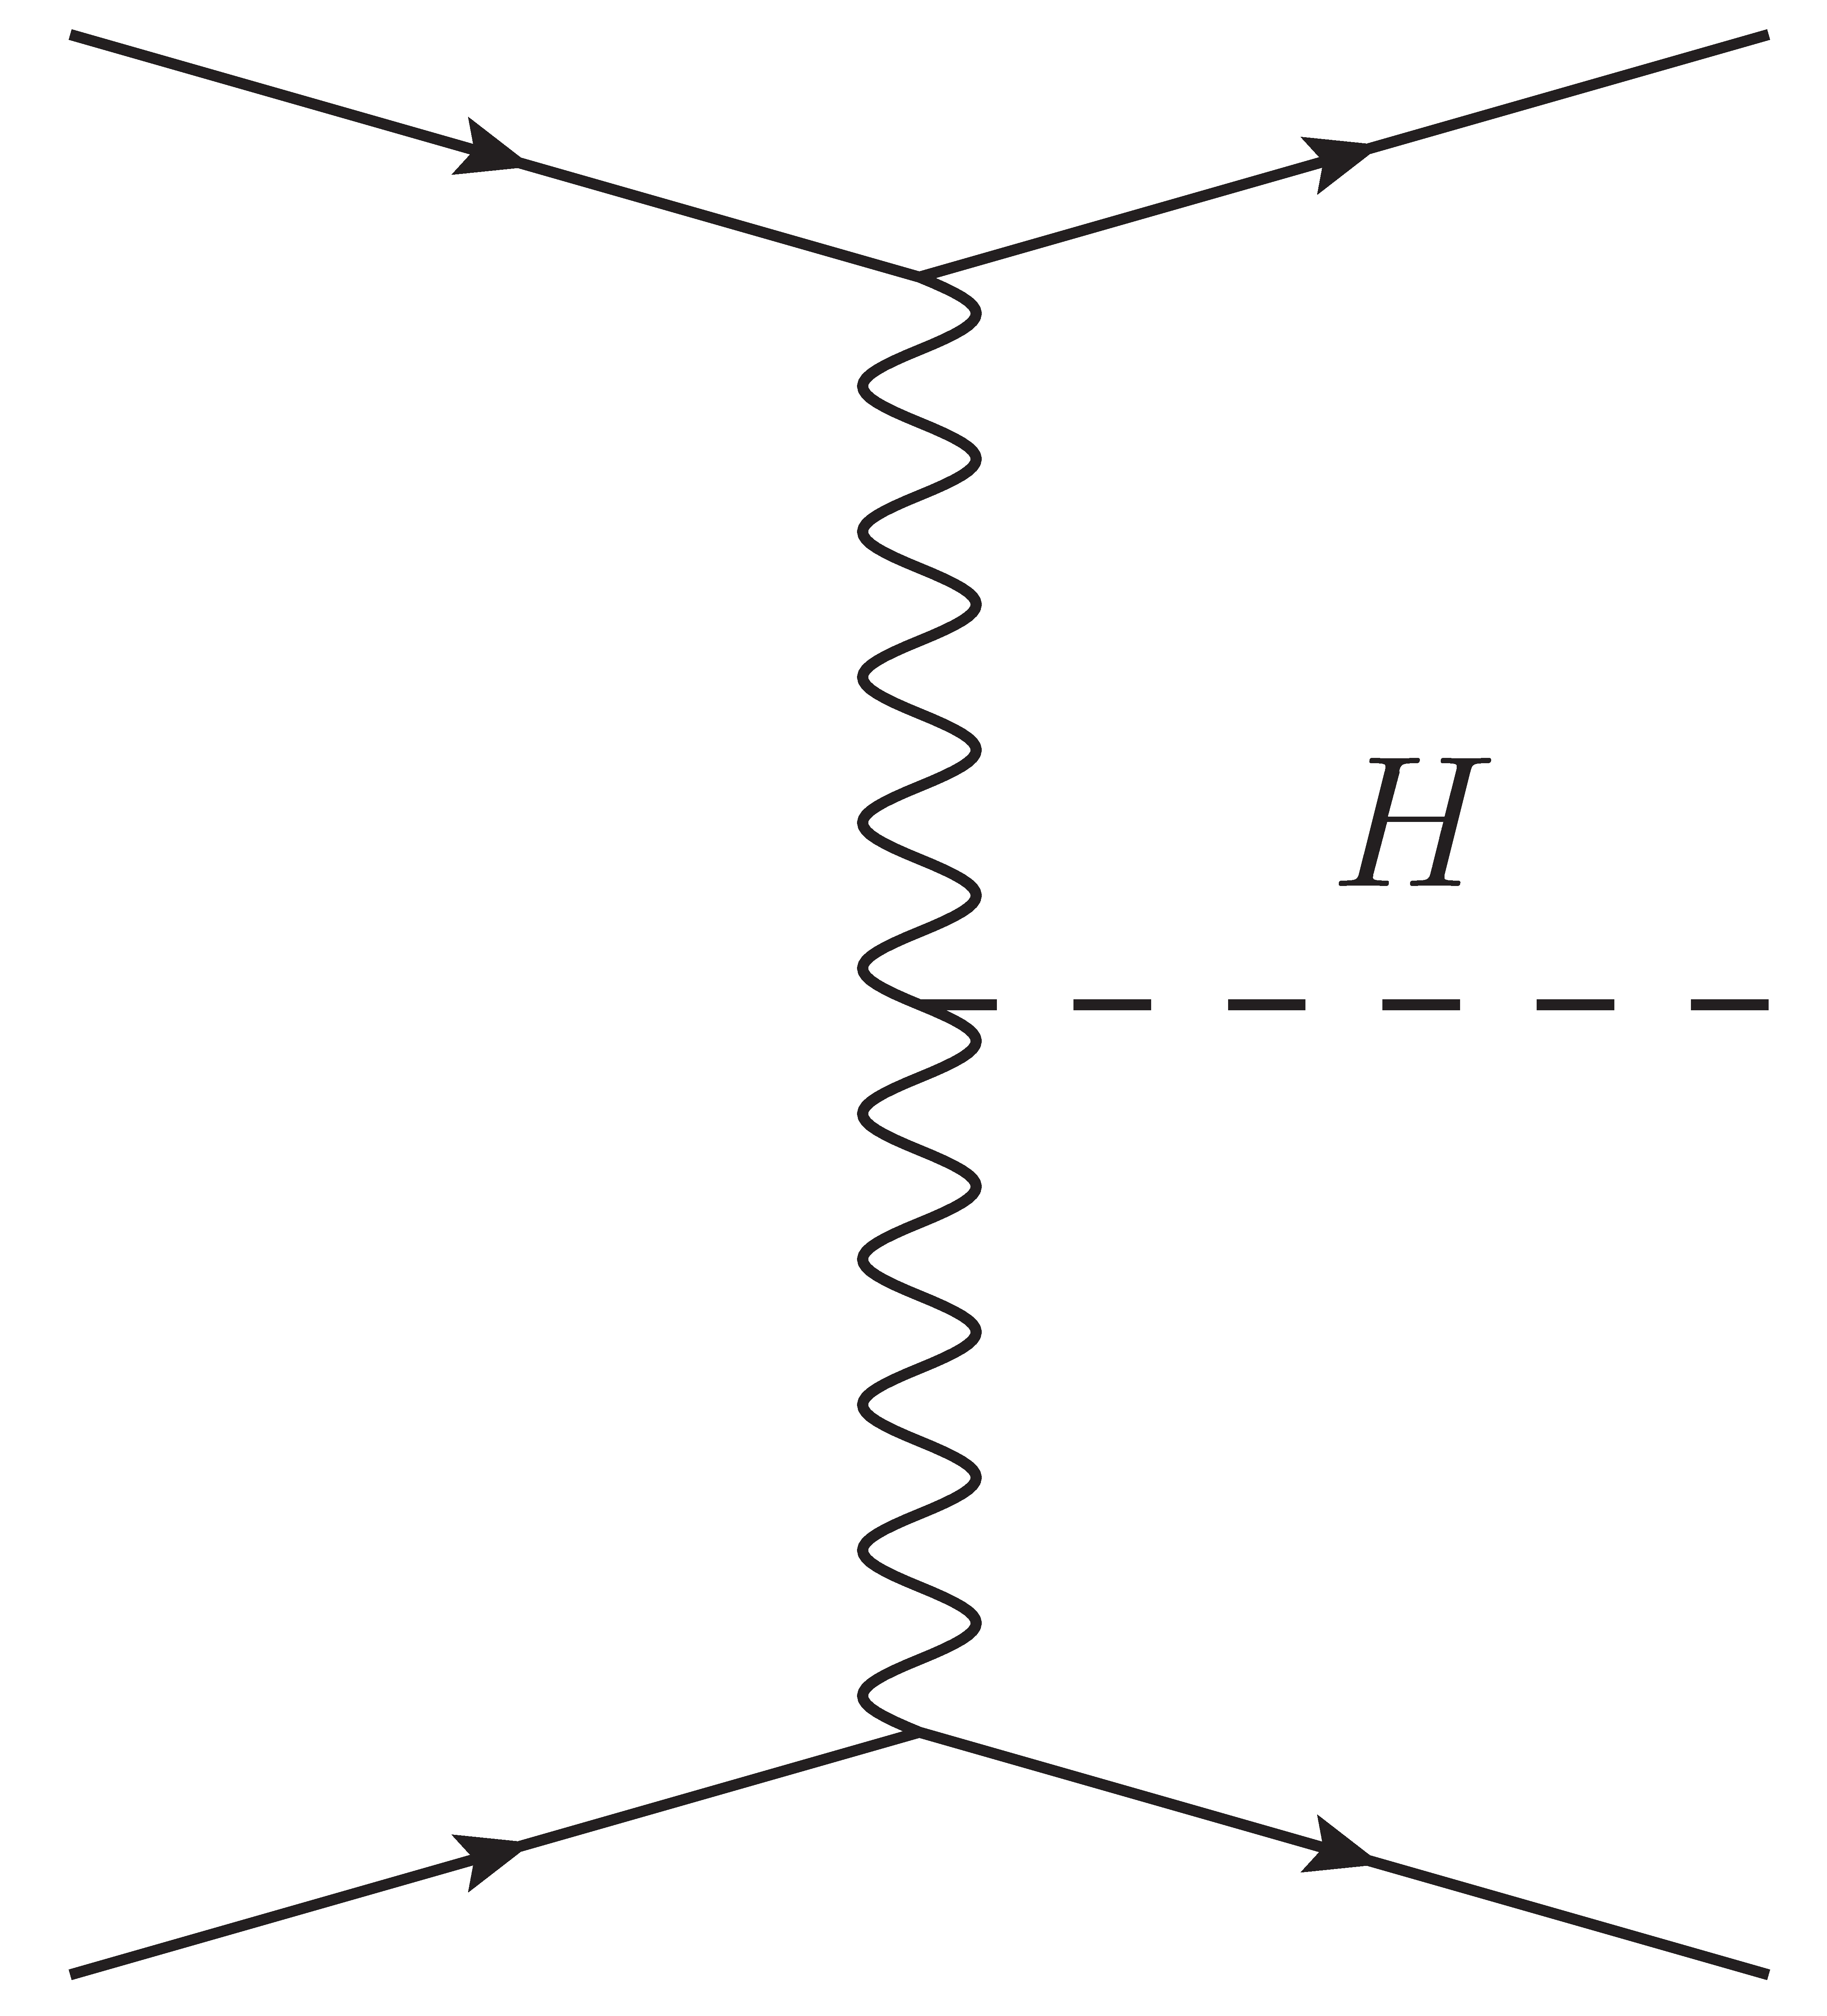
\includegraphics[scale=0.3]{../figs/VBF_H.png}
    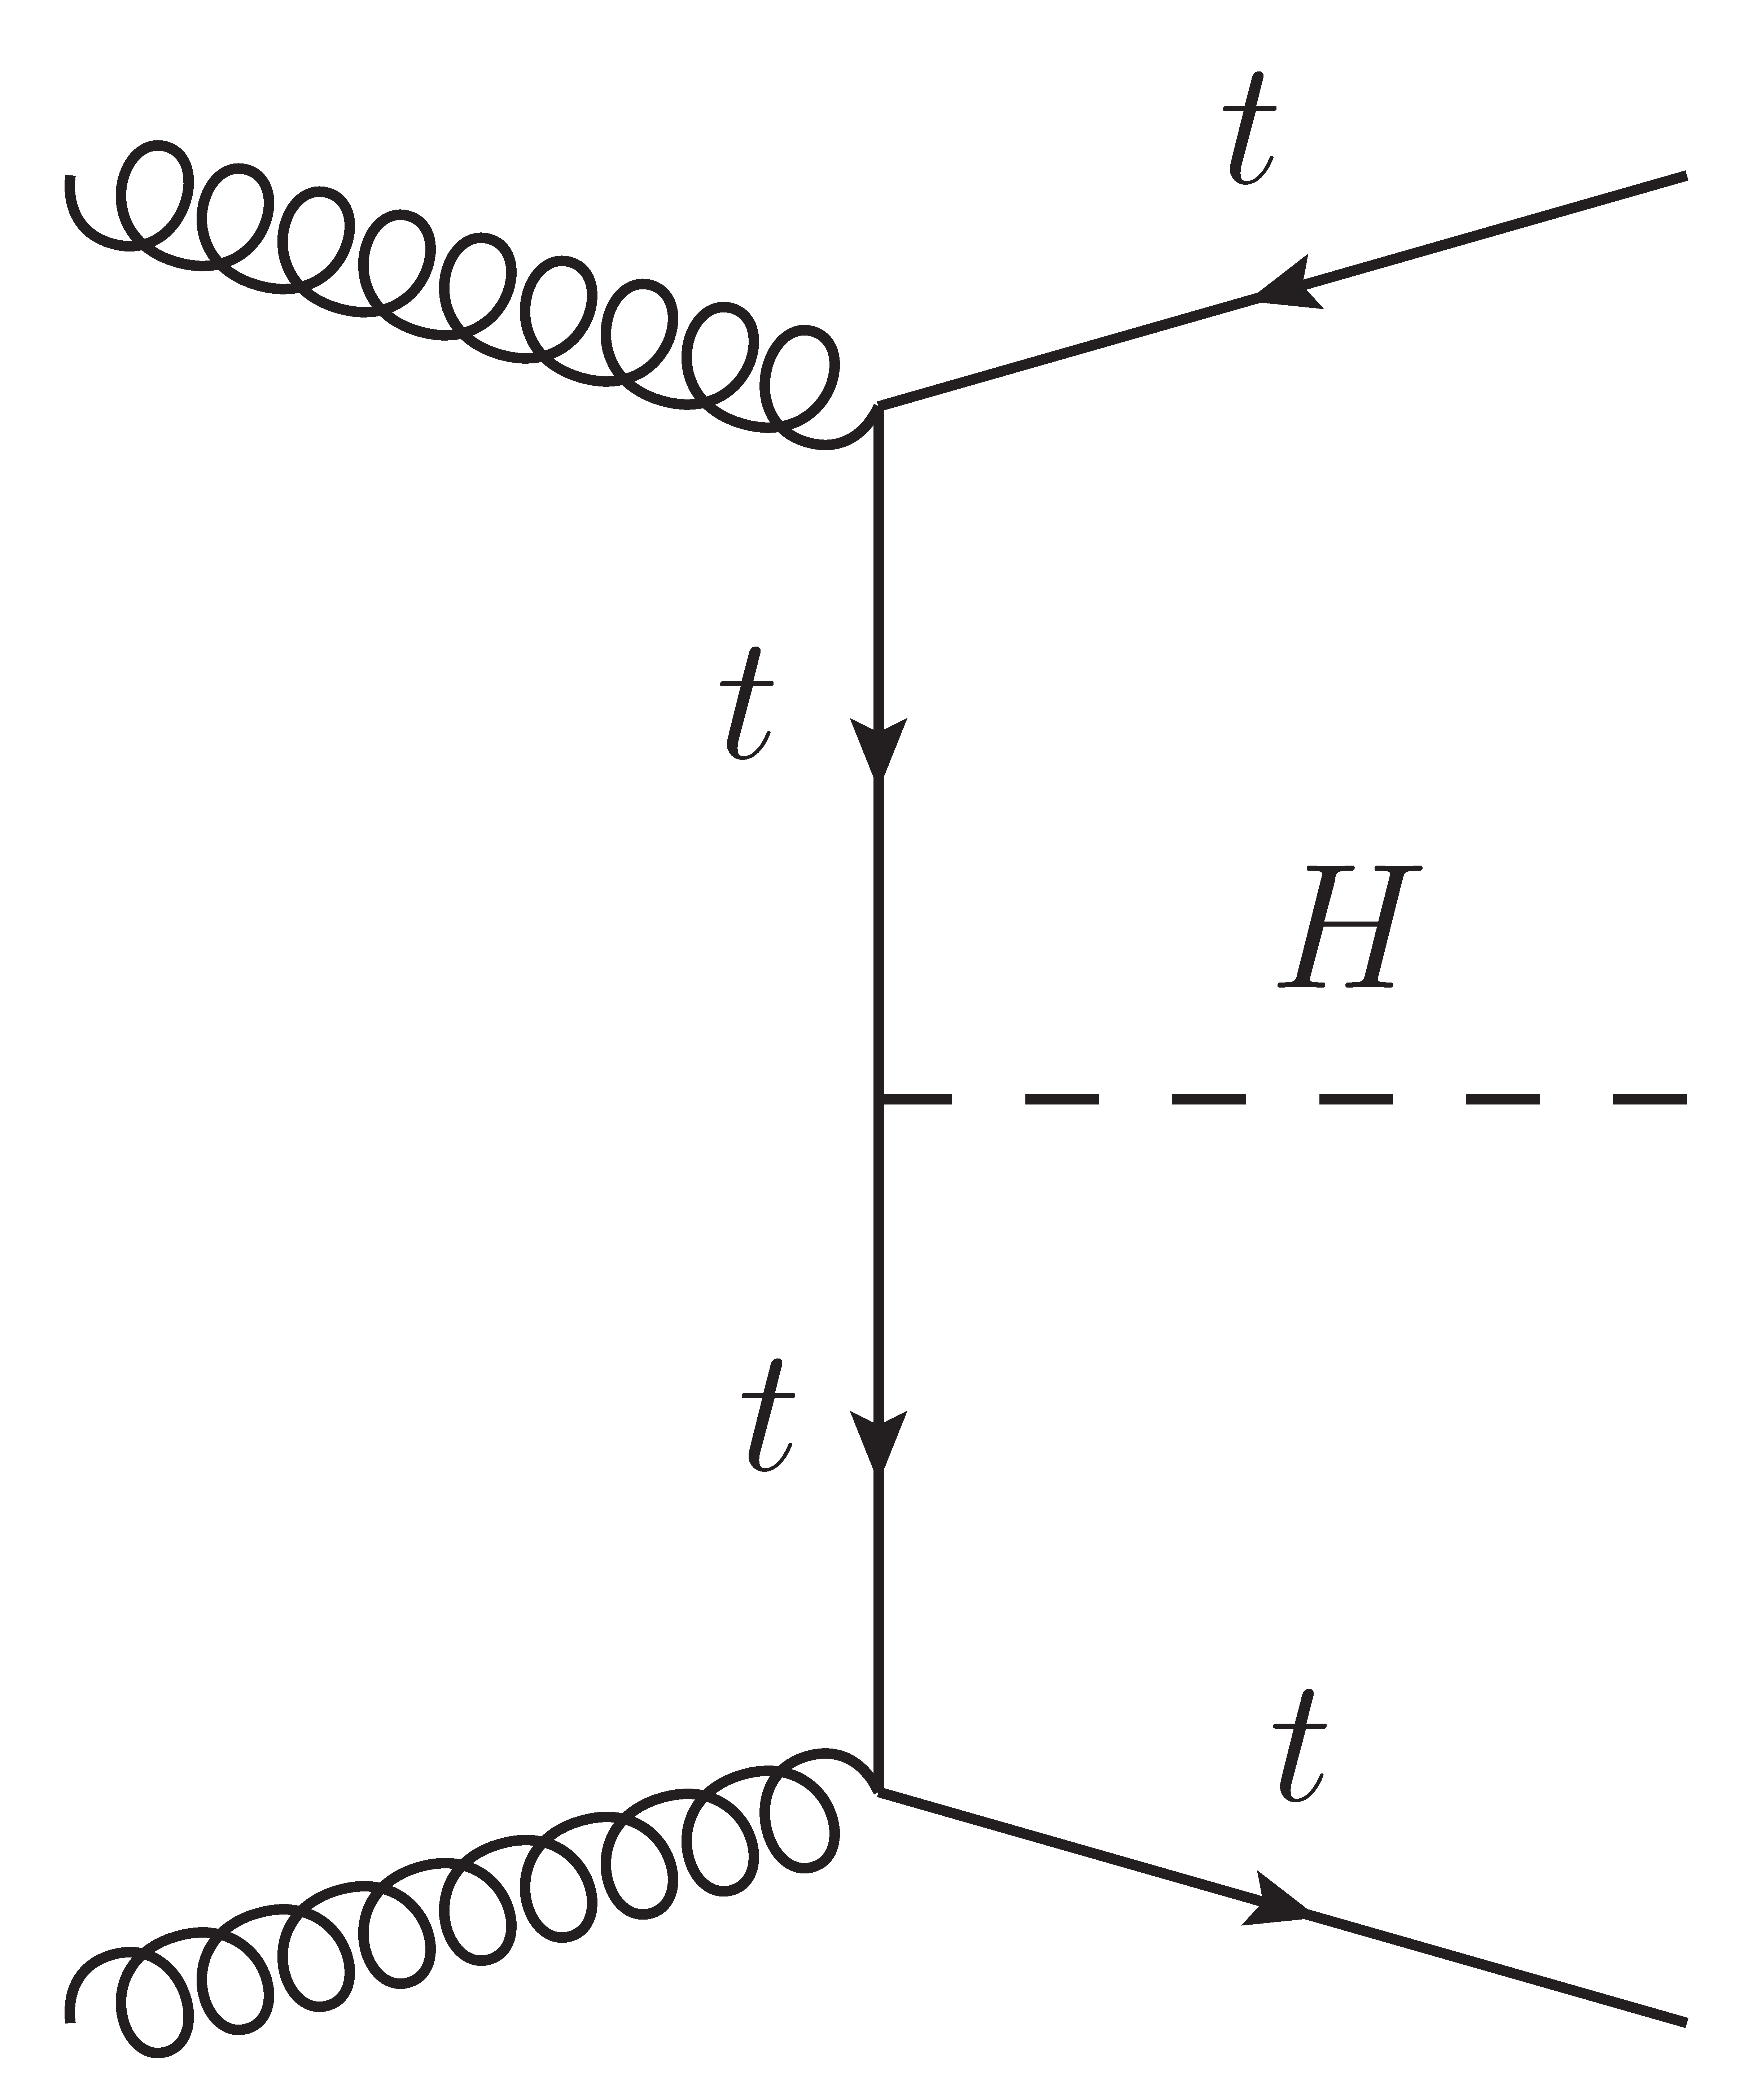
\includegraphics[scale=0.3]{../figs/QuarkF_H.png}
    %\caption{Higgs boson production Feynman diagrams for proton-proton collisions: gluon fusion [left-up], Higgsstrahlung [right-up], vector boson fusion [left-down] and quark fusion [right-down].}
    %\label{fig:HiggsProd}
  \end{center}
\end{figure}

\vspace{-.2cm}
    \begin{block}{}
      \tiny \centering Higgs boson production Feynman diagrams for proton-proton collisions: gluon fusion [left-up], Higgsstrahlung [right-up], vector boson fusion [left-down] and quark fusion [right-down].
    \end{block}

\end{frame}

\begin{frame}{}
\vspace{-.2cm}
\begin{figure}[!Hhtbp]
  \begin{center}
    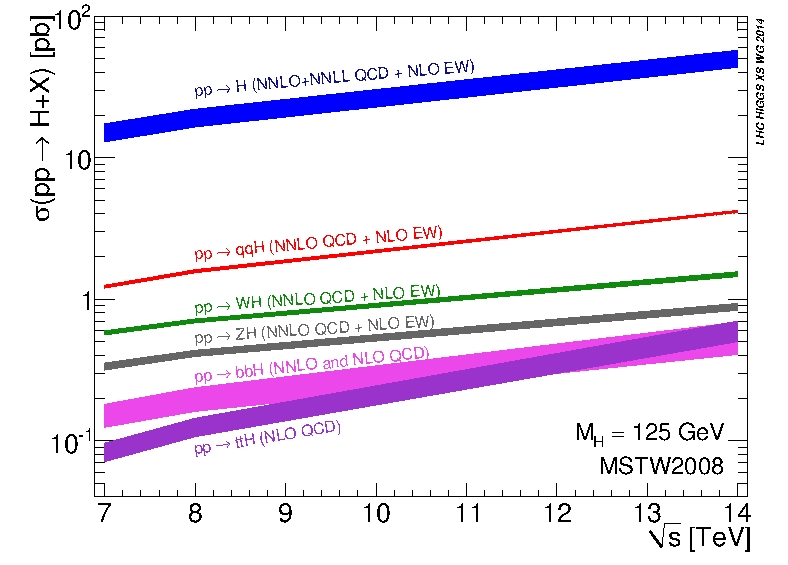
\includegraphics[width=0.6\textwidth]{../figs/7-14_Higgs_xsec.jpg}
    %\caption{Higgs boson theoretical production cross section as a function of center of mass energy, for a Higgs boson mass of 125 GeV/$c^{2}$~\cite{HIGGSXSWG}.}
    %\label{fig:HiggsProdXS}
  \end{center}
\end{figure}

\vspace{-.2cm}
    \begin{block}{}
      \tiny \centering Higgs boson theoretical production cross section as a function of center of mass energy, for a Higgs boson mass of 125 GeV/$c^{2}$.
    \end{block}

\end{frame}

\begin{frame}{Higgs decay}
\vspace{-.2cm}
\begin{figure}[!Hhtbp]
  \begin{center}
    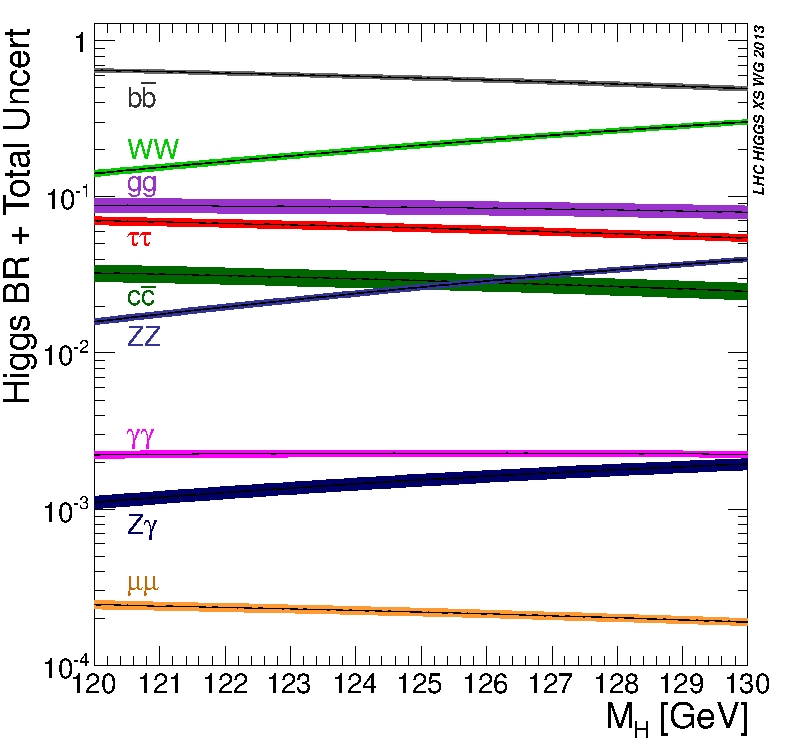
\includegraphics[width=0.6\textwidth]{../figs/Higgs_BR_120-130.jpg}
    %\caption{Higgs boson decay branching ratios as a function of its mass~\cite{Dittmaier:2011ti, Dittmaier:2012vm, Heinemeyer:2013tqa, HIGGSXSWG}.}
    %\label{fig:HiggsBrs}
  \end{center}
\end{figure}

\vspace{-.2cm}
    \begin{block}{}
      \tiny \centering Higgs boson decay branching ratios as a function of its mass.
    \end{block}

\end{frame}

\begin{frame}{}
\vspace{-.2cm}
\begin{figure}[!Hhtbp]
  \begin{center}
    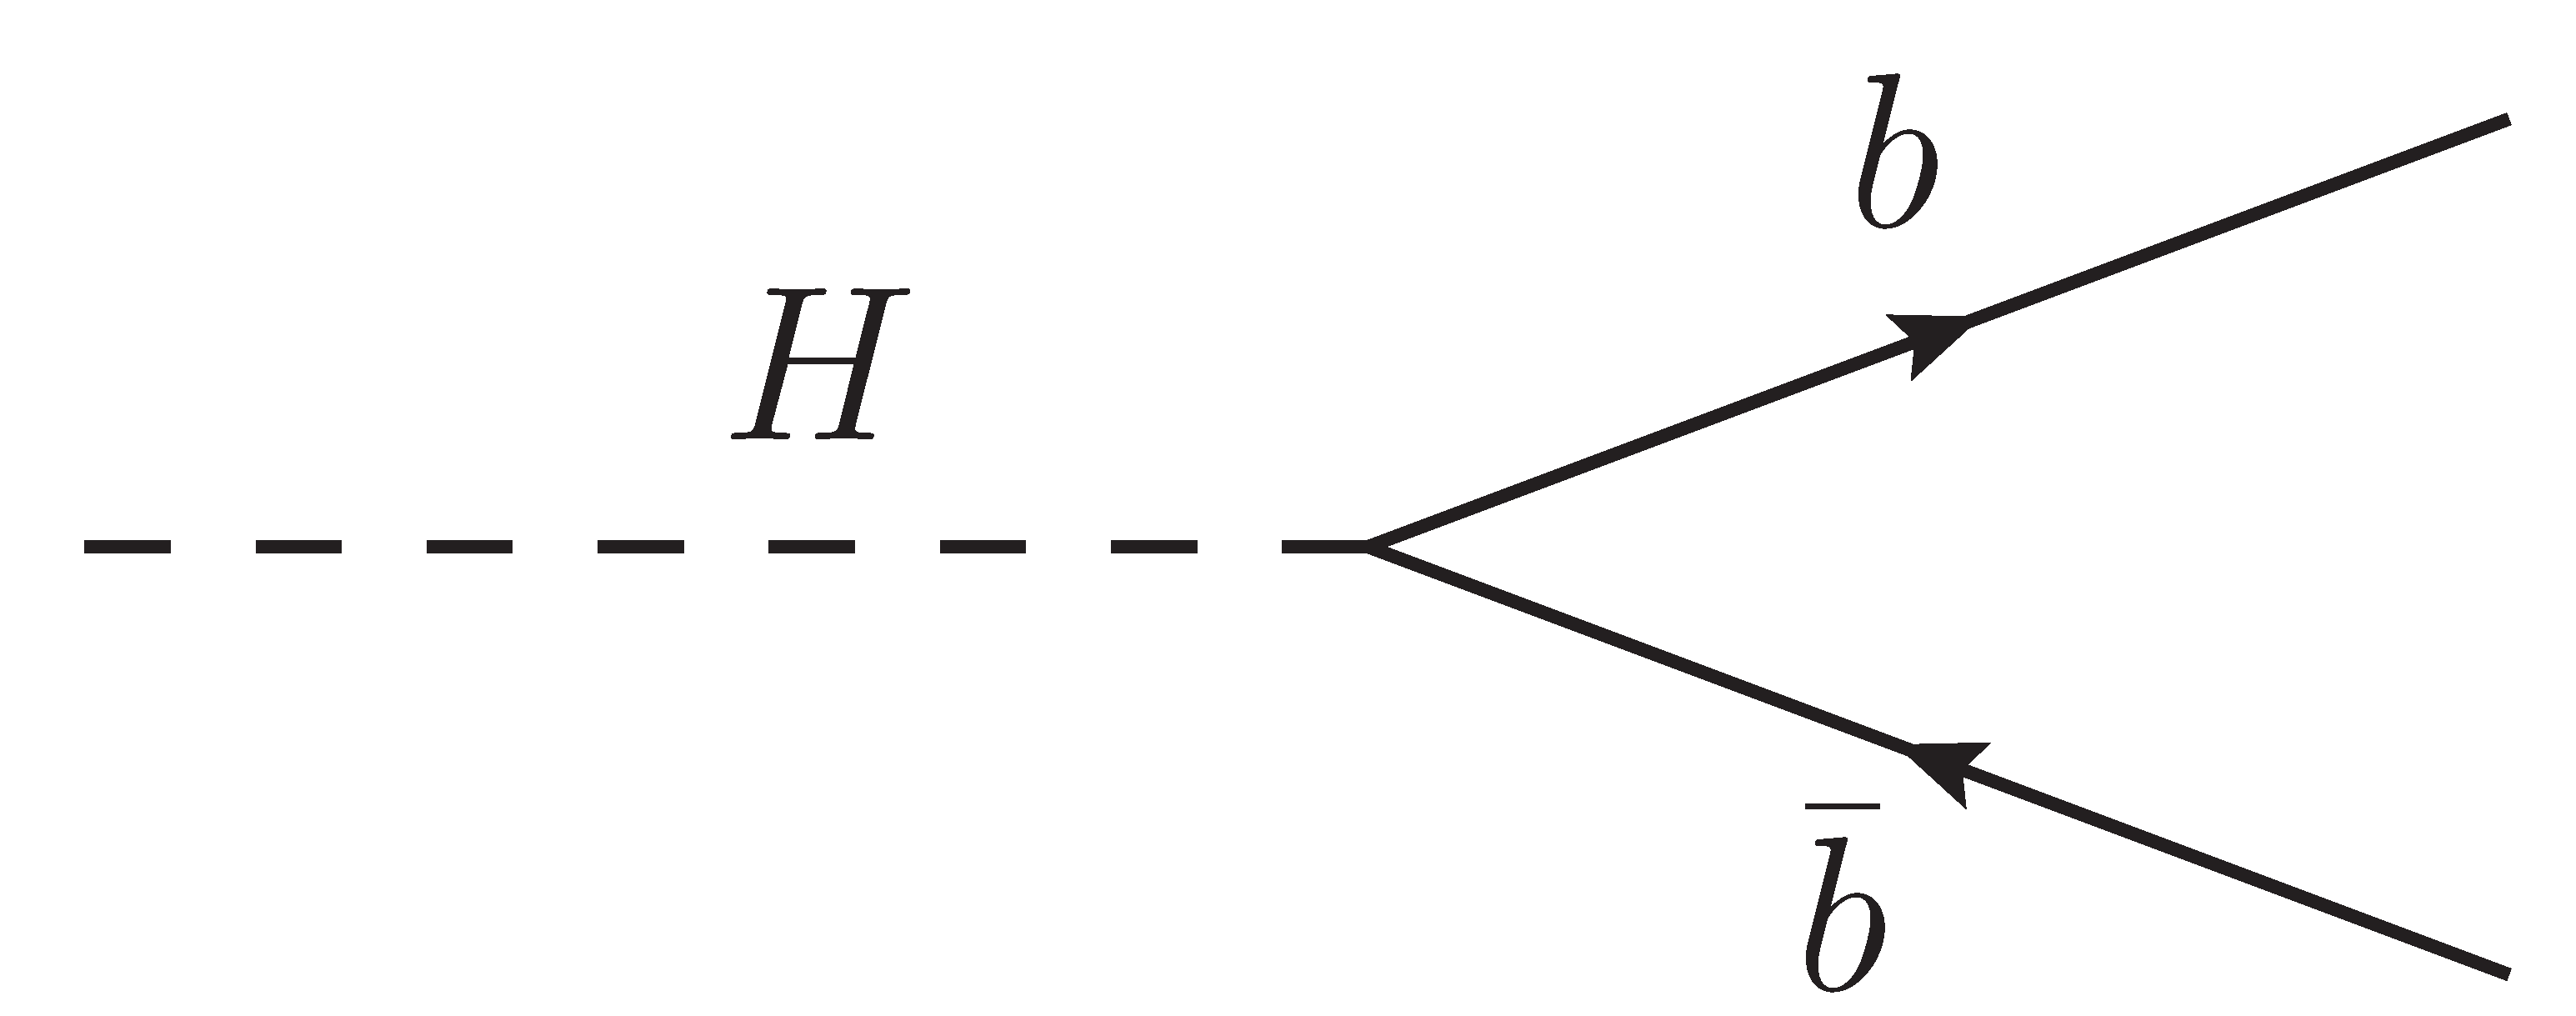
\includegraphics[width=0.3\textwidth]{../figs/BB_H.png}
    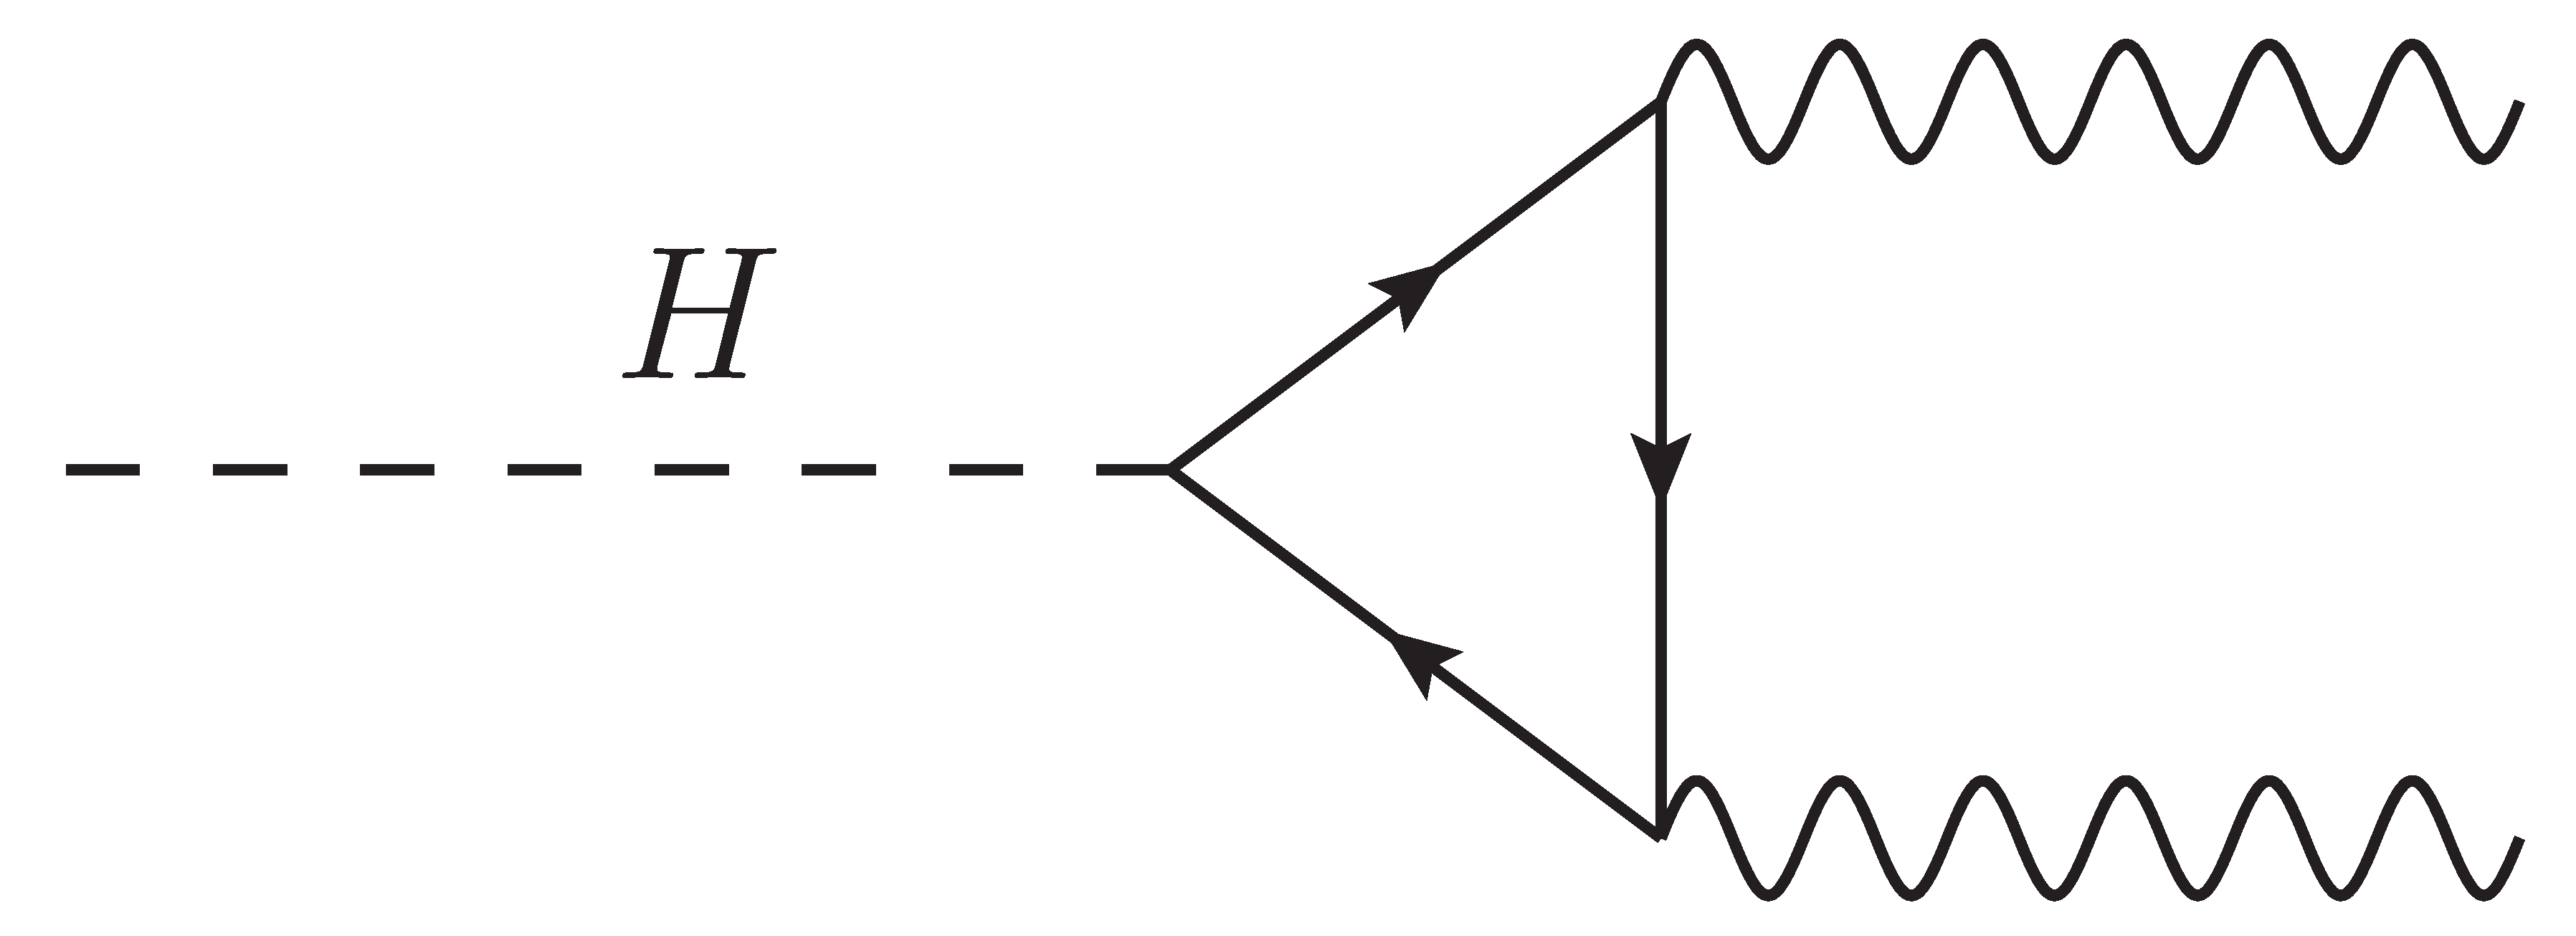
\includegraphics[width=0.3\textwidth]{../figs/Diphoton_H.png}
    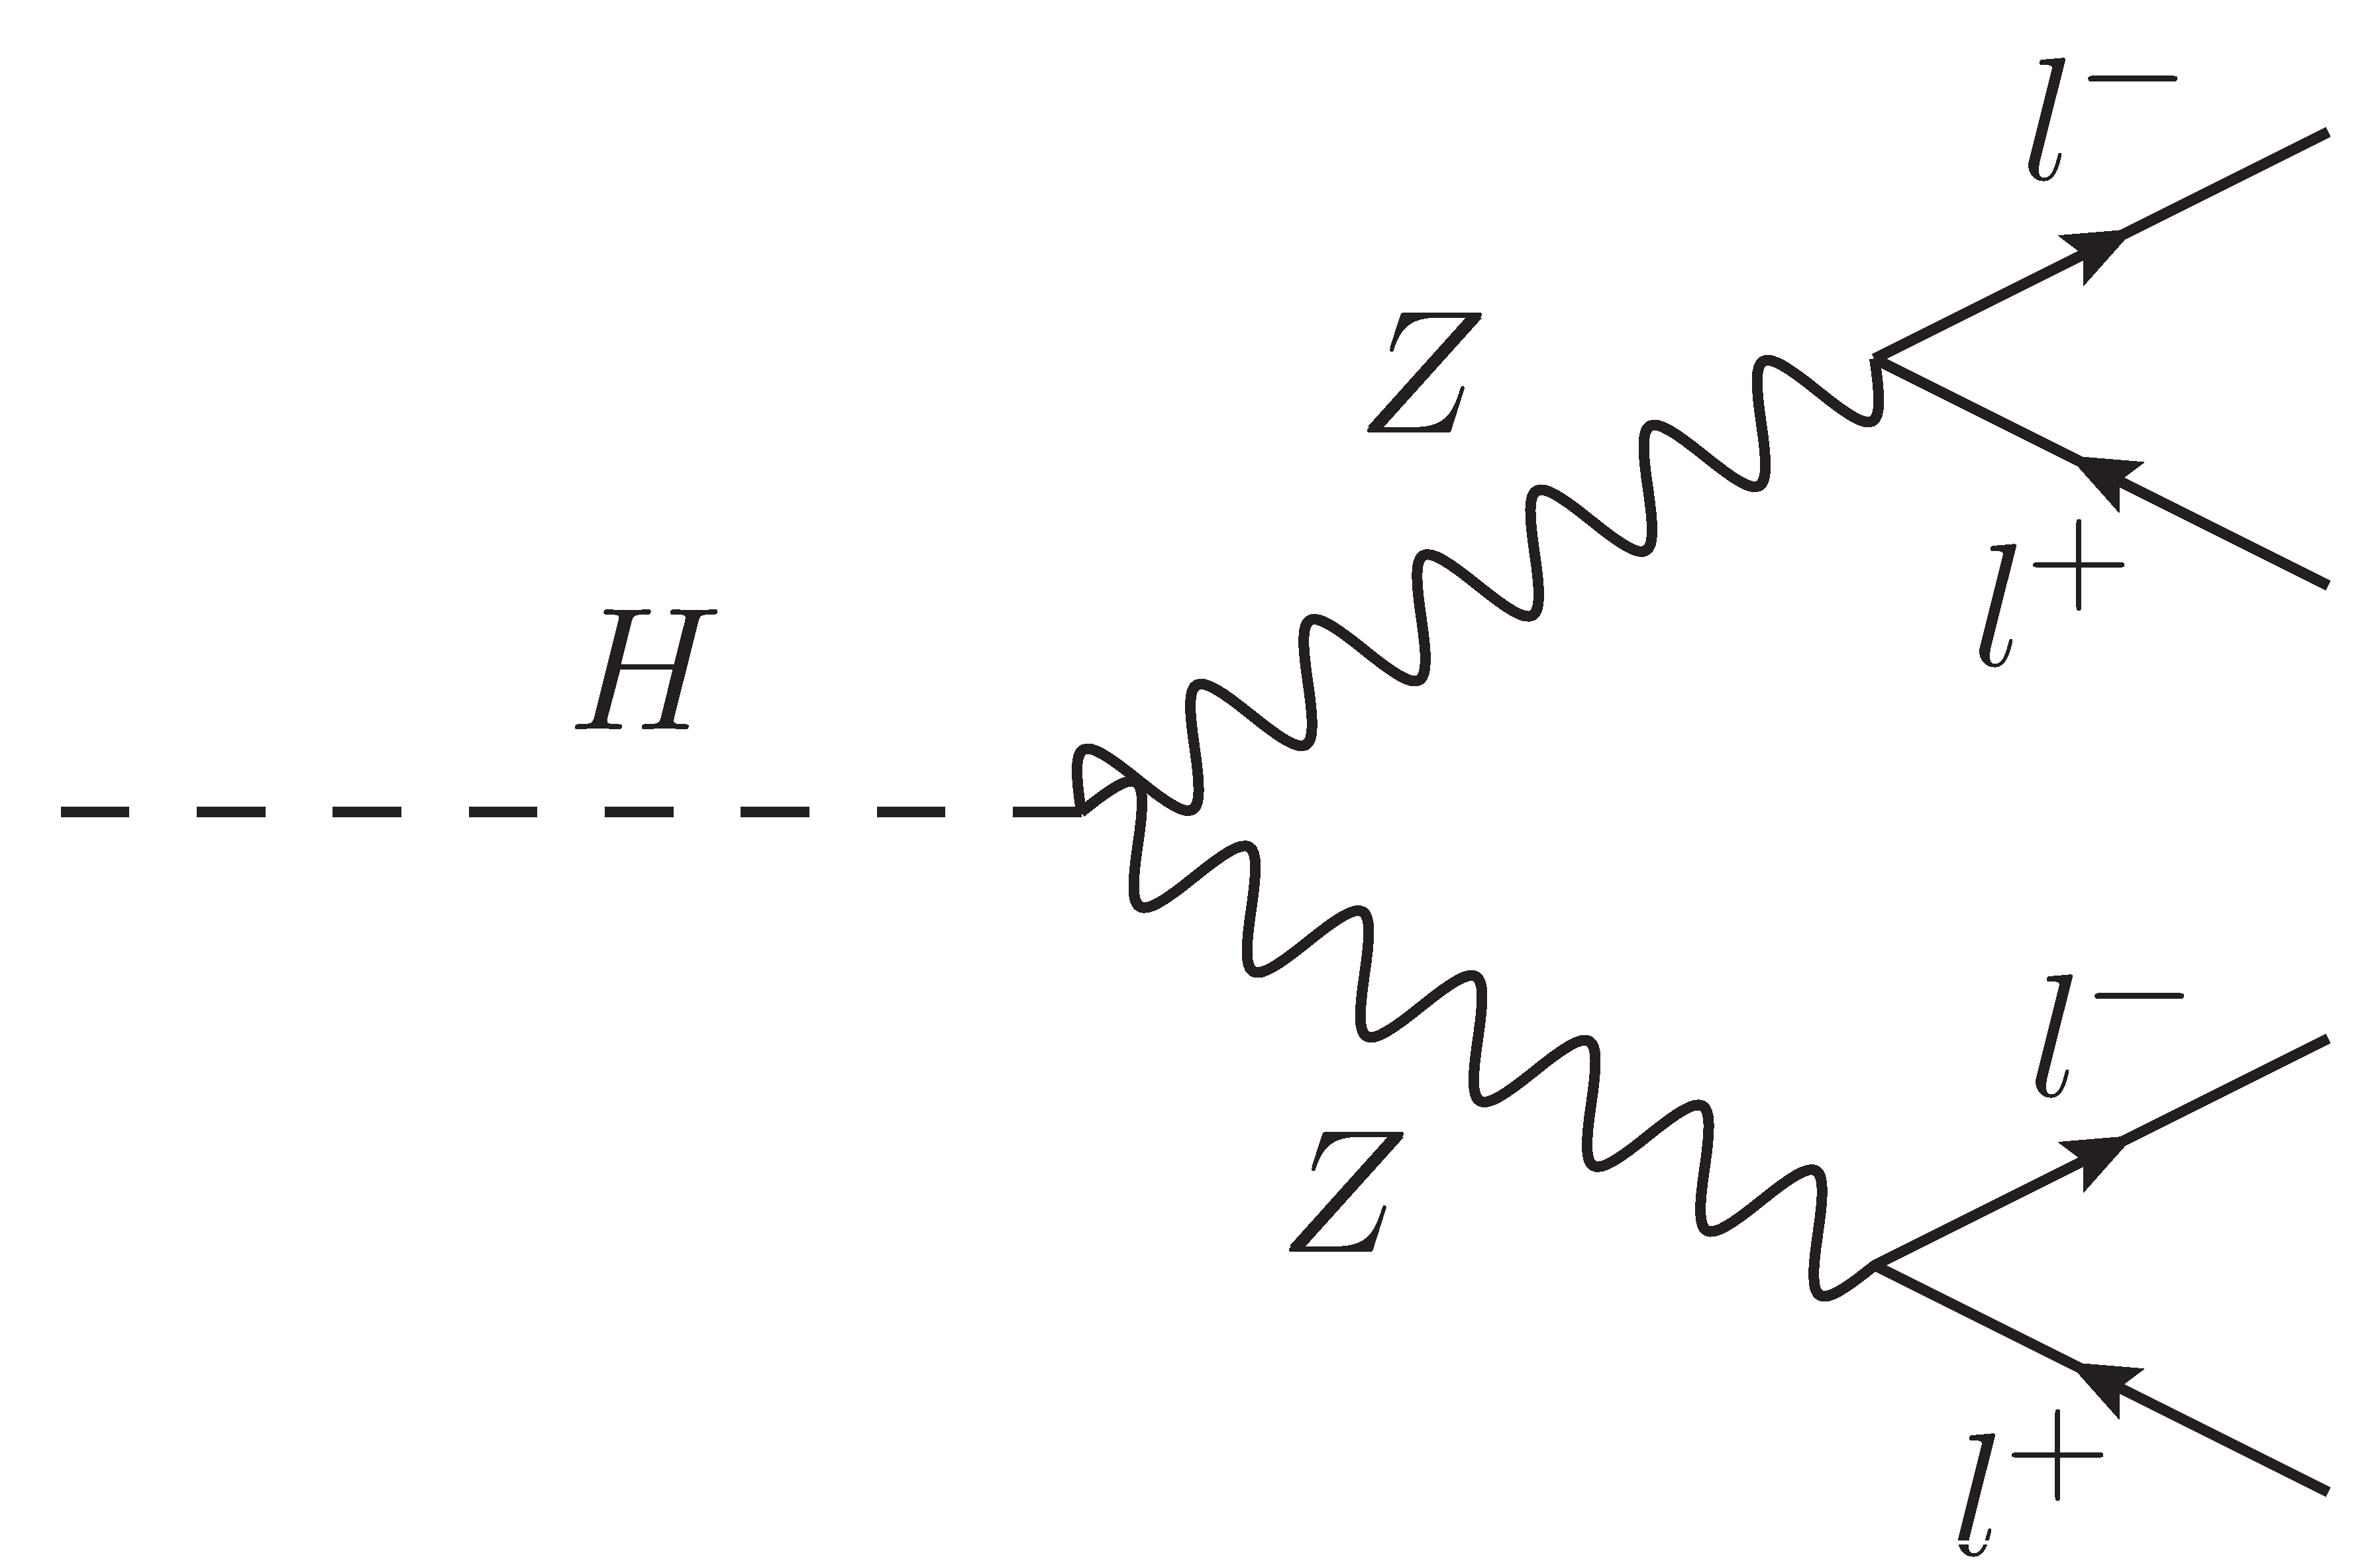
\includegraphics[width=0.3\textwidth]{../figs/Golden_H.png}
    %\caption{Feynman diagrams of Higgs boson decay: $b\bar{b}$ [left], diphoton [center] and golden channels [right].}
    %\label{fig:HiggsDecays}
  \end{center}
\end{figure}

\vspace{-.2cm}
    \begin{block}{}
      \tiny \centering Feynman diagrams of Higgs boson decay: $b\bar{b}$ [left], diphoton [center] and golden channels [right].
    \end{block}

\end{frame}

\begin{frame}{Higgs mass}
\vspace{-.2cm}
\begin{figure}[!Hhtbp]
  \begin{center}
    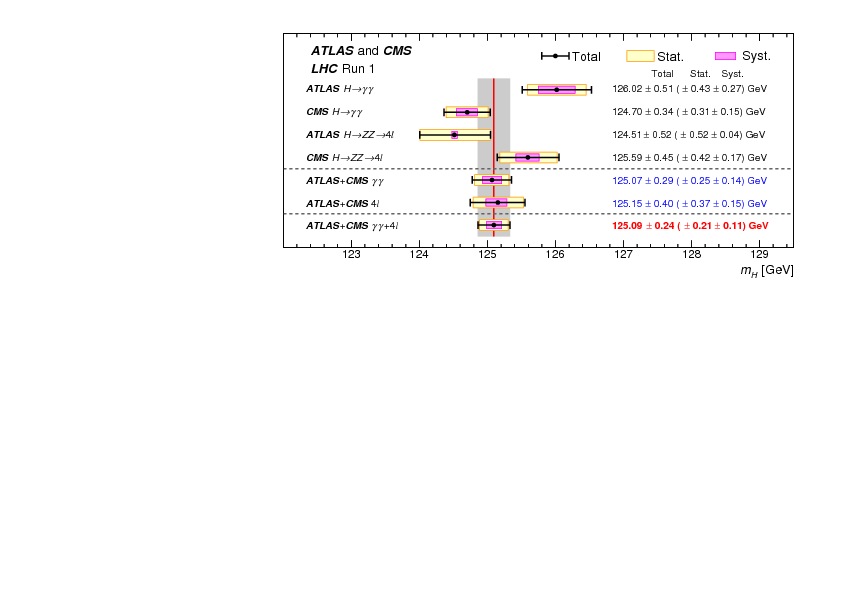
\includegraphics[trim=10cm 7cm 1cm 1cm, clip=true, width=0.8\textwidth]{../figs/LHC_combined_obs_unblind_summary_a1_final.png}
    %\caption{ATLAS and CMS combination of Higgs boson mass measurement [top] and $\sigma/\sigma_{SM}$ (measured cross section over theoretical SM cross section) for searches performed by ATLAS and CMS in different Higgs boson decay channels [bottom]~\cite{Aad:2015zhl,CMS:2014ega,ATLAS-CONF-2015-007}.}
    %\label{fig:HiggsMass}
  \end{center}
\end{figure}

\vspace{-.2cm}
    \begin{block}{}
      \tiny \centering ATLAS and CMS combination of Higgs boson mass measurement.
    \end{block}

\end{frame}

\begin{frame}{}
\vspace{-.2cm}
\begin{figure}[!Hhtbp]
  \begin{center}
    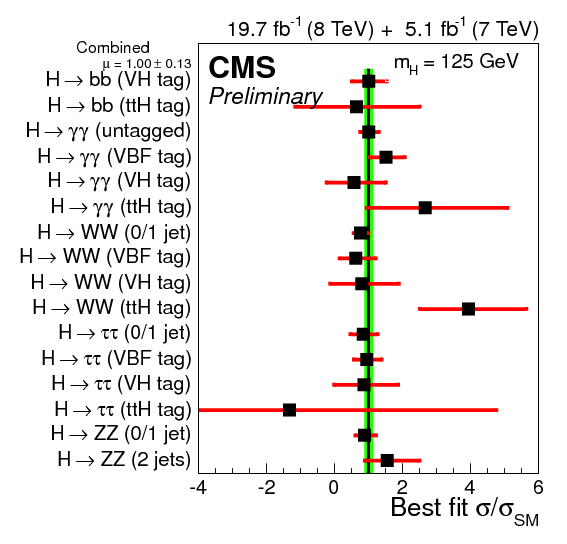
\includegraphics[width=0.5\textwidth]{../figs/sqr_mlz_ccc_mH125.png}
    \includegraphics[width=0.4\textwidth]{../figs/ATLAS_HIGGS_mu_Summary.png}
    %\caption{ATLAS and CMS combination of Higgs boson mass measurement [top] and $\sigma/\sigma_{SM}$ (measured cross section over theoretical SM cross section) for searches performed by ATLAS and CMS in different Higgs boson decay channels [bottom]~\cite{Aad:2015zhl,CMS:2014ega,ATLAS-CONF-2015-007}.}
    %\label{fig:HiggsMass}
  \end{center}
\end{figure}

\vspace{-.2cm}
    \begin{block}{}
      \tiny \centering $\sigma/\sigma_{SM}$ (measured cross section over theoretical SM cross section) for searches performed by ATLAS and CMS in different Higgs boson decay channels.
    \end{block}

\end{frame}

\begin{frame}{Higgs width}
\vspace{-.2cm}
\begin{figure}[!Hhtbp]
  \begin{center}
    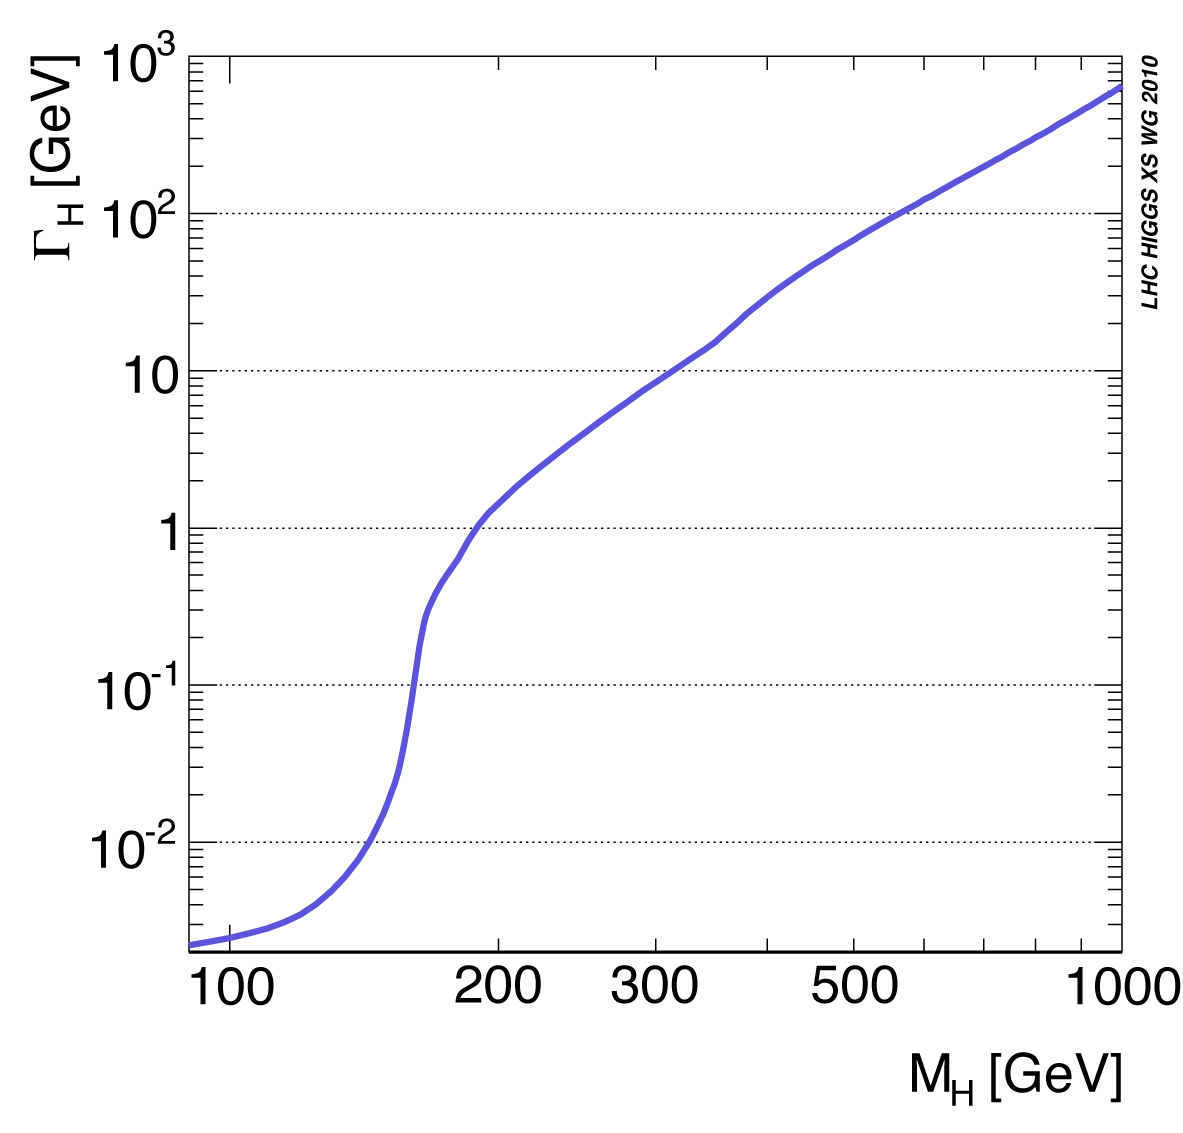
\includegraphics[width=0.42\textwidth]{../figs/u0g5o.png}
    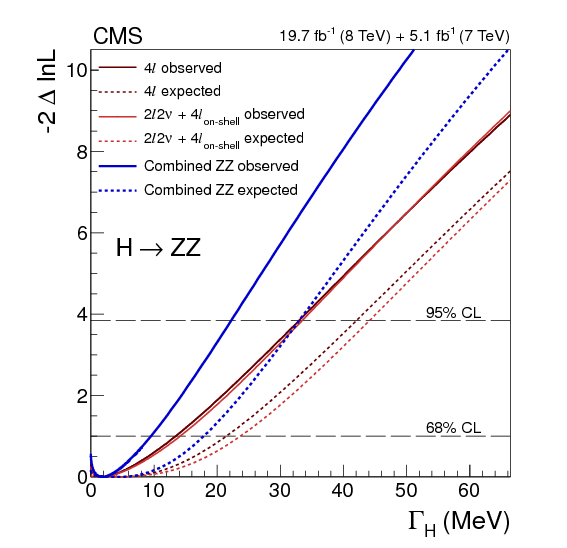
\includegraphics[width=0.42\textwidth]{../figs/AllFitPaper_30_04_14_MeV.png}
    %\caption{Higgs boson width as a function of its mass~\cite{Dittmaier:2011ti, Dittmaier:2012vm, Heinemeyer:2013tqa, HIGGSXSWG} [left] and current limits from CMS measurement~\cite{Khachatryan:2014iha} [right].}
    %\label{fig:WidthHiggs}
  \end{center}
\end{figure}

\vspace{-.2cm}
    \begin{block}{}
      \tiny \centering Higgs boson width as a function of its mass [left] and current limits from CMS measurement [right].
    \end{block}

\end{frame}

%\begin{frame}{}
%\vspace{-.2cm}
%
%\vspace{-.2cm}
%    \begin{block}{}
%      \tiny \centering 
%    \end{block}
%
%\end{frame}